\documentclass[10pt,conference]{IEEEtran}
\usepackage{cite}
\usepackage{amsmath,amssymb,amsfonts}
\usepackage{algorithmic}
\usepackage{graphicx}
\usepackage{textcomp}
\usepackage{xcolor}
\usepackage[hyphens]{url}
\usepackage{fancyhdr}
\usepackage{hyperref}
\usepackage{inconsolata}
\usepackage{flushend}


% Ensure letter paper
\pdfpagewidth=8.5in
\pdfpageheight=11in

\newcommand{\hpcayear}{2025}


%
\setlength\unitlength{1mm}
\newcommand{\twodots}{\mathinner {\ldotp \ldotp}}
% bb font symbols
\newcommand{\Rho}{\mathrm{P}}
\newcommand{\Tau}{\mathrm{T}}

\newfont{\bbb}{msbm10 scaled 700}
\newcommand{\CCC}{\mbox{\bbb C}}

\newfont{\bb}{msbm10 scaled 1100}
\newcommand{\CC}{\mbox{\bb C}}
\newcommand{\PP}{\mbox{\bb P}}
\newcommand{\RR}{\mbox{\bb R}}
\newcommand{\QQ}{\mbox{\bb Q}}
\newcommand{\ZZ}{\mbox{\bb Z}}
\newcommand{\FF}{\mbox{\bb F}}
\newcommand{\GG}{\mbox{\bb G}}
\newcommand{\EE}{\mbox{\bb E}}
\newcommand{\NN}{\mbox{\bb N}}
\newcommand{\KK}{\mbox{\bb K}}
\newcommand{\HH}{\mbox{\bb H}}
\newcommand{\SSS}{\mbox{\bb S}}
\newcommand{\UU}{\mbox{\bb U}}
\newcommand{\VV}{\mbox{\bb V}}


\newcommand{\yy}{\mathbbm{y}}
\newcommand{\xx}{\mathbbm{x}}
\newcommand{\zz}{\mathbbm{z}}
\newcommand{\sss}{\mathbbm{s}}
\newcommand{\rr}{\mathbbm{r}}
\newcommand{\pp}{\mathbbm{p}}
\newcommand{\qq}{\mathbbm{q}}
\newcommand{\ww}{\mathbbm{w}}
\newcommand{\hh}{\mathbbm{h}}
\newcommand{\vvv}{\mathbbm{v}}

% Vectors

\newcommand{\av}{{\bf a}}
\newcommand{\bv}{{\bf b}}
\newcommand{\cv}{{\bf c}}
\newcommand{\dv}{{\bf d}}
\newcommand{\ev}{{\bf e}}
\newcommand{\fv}{{\bf f}}
\newcommand{\gv}{{\bf g}}
\newcommand{\hv}{{\bf h}}
\newcommand{\iv}{{\bf i}}
\newcommand{\jv}{{\bf j}}
\newcommand{\kv}{{\bf k}}
\newcommand{\lv}{{\bf l}}
\newcommand{\mv}{{\bf m}}
\newcommand{\nv}{{\bf n}}
\newcommand{\ov}{{\bf o}}
\newcommand{\pv}{{\bf p}}
\newcommand{\qv}{{\bf q}}
\newcommand{\rv}{{\bf r}}
\newcommand{\sv}{{\bf s}}
\newcommand{\tv}{{\bf t}}
\newcommand{\uv}{{\bf u}}
\newcommand{\wv}{{\bf w}}
\newcommand{\vv}{{\bf v}}
\newcommand{\xv}{{\bf x}}
\newcommand{\yv}{{\bf y}}
\newcommand{\zv}{{\bf z}}
\newcommand{\zerov}{{\bf 0}}
\newcommand{\onev}{{\bf 1}}

% Matrices

\newcommand{\Am}{{\bf A}}
\newcommand{\Bm}{{\bf B}}
\newcommand{\Cm}{{\bf C}}
\newcommand{\Dm}{{\bf D}}
\newcommand{\Em}{{\bf E}}
\newcommand{\Fm}{{\bf F}}
\newcommand{\Gm}{{\bf G}}
\newcommand{\Hm}{{\bf H}}
\newcommand{\Id}{{\bf I}}
\newcommand{\Jm}{{\bf J}}
\newcommand{\Km}{{\bf K}}
\newcommand{\Lm}{{\bf L}}
\newcommand{\Mm}{{\bf M}}
\newcommand{\Nm}{{\bf N}}
\newcommand{\Om}{{\bf O}}
\newcommand{\Pm}{{\bf P}}
\newcommand{\Qm}{{\bf Q}}
\newcommand{\Rm}{{\bf R}}
\newcommand{\Sm}{{\bf S}}
\newcommand{\Tm}{{\bf T}}
\newcommand{\Um}{{\bf U}}
\newcommand{\Wm}{{\bf W}}
\newcommand{\Vm}{{\bf V}}
\newcommand{\Xm}{{\bf X}}
\newcommand{\Ym}{{\bf Y}}
\newcommand{\Zm}{{\bf Z}}

% Calligraphic

\newcommand{\Ac}{{\cal A}}
\newcommand{\Bc}{{\cal B}}
\newcommand{\Cc}{{\cal C}}
\newcommand{\Dc}{{\cal D}}
\newcommand{\Ec}{{\cal E}}
\newcommand{\Fc}{{\cal F}}
\newcommand{\Gc}{{\cal G}}
\newcommand{\Hc}{{\cal H}}
\newcommand{\Ic}{{\cal I}}
\newcommand{\Jc}{{\cal J}}
\newcommand{\Kc}{{\cal K}}
\newcommand{\Lc}{{\cal L}}
\newcommand{\Mc}{{\cal M}}
\newcommand{\Nc}{{\cal N}}
\newcommand{\nc}{{\cal n}}
\newcommand{\Oc}{{\cal O}}
\newcommand{\Pc}{{\cal P}}
\newcommand{\Qc}{{\cal Q}}
\newcommand{\Rc}{{\cal R}}
\newcommand{\Sc}{{\cal S}}
\newcommand{\Tc}{{\cal T}}
\newcommand{\Uc}{{\cal U}}
\newcommand{\Wc}{{\cal W}}
\newcommand{\Vc}{{\cal V}}
\newcommand{\Xc}{{\cal X}}
\newcommand{\Yc}{{\cal Y}}
\newcommand{\Zc}{{\cal Z}}

% Bold greek letters

\newcommand{\alphav}{\hbox{\boldmath$\alpha$}}
\newcommand{\betav}{\hbox{\boldmath$\beta$}}
\newcommand{\gammav}{\hbox{\boldmath$\gamma$}}
\newcommand{\deltav}{\hbox{\boldmath$\delta$}}
\newcommand{\etav}{\hbox{\boldmath$\eta$}}
\newcommand{\lambdav}{\hbox{\boldmath$\lambda$}}
\newcommand{\epsilonv}{\hbox{\boldmath$\epsilon$}}
\newcommand{\nuv}{\hbox{\boldmath$\nu$}}
\newcommand{\muv}{\hbox{\boldmath$\mu$}}
\newcommand{\zetav}{\hbox{\boldmath$\zeta$}}
\newcommand{\phiv}{\hbox{\boldmath$\phi$}}
\newcommand{\psiv}{\hbox{\boldmath$\psi$}}
\newcommand{\thetav}{\hbox{\boldmath$\theta$}}
\newcommand{\tauv}{\hbox{\boldmath$\tau$}}
\newcommand{\omegav}{\hbox{\boldmath$\omega$}}
\newcommand{\xiv}{\hbox{\boldmath$\xi$}}
\newcommand{\sigmav}{\hbox{\boldmath$\sigma$}}
\newcommand{\piv}{\hbox{\boldmath$\pi$}}
\newcommand{\rhov}{\hbox{\boldmath$\rho$}}
\newcommand{\upsilonv}{\hbox{\boldmath$\upsilon$}}

\newcommand{\Gammam}{\hbox{\boldmath$\Gamma$}}
\newcommand{\Lambdam}{\hbox{\boldmath$\Lambda$}}
\newcommand{\Deltam}{\hbox{\boldmath$\Delta$}}
\newcommand{\Sigmam}{\hbox{\boldmath$\Sigma$}}
\newcommand{\Phim}{\hbox{\boldmath$\Phi$}}
\newcommand{\Pim}{\hbox{\boldmath$\Pi$}}
\newcommand{\Psim}{\hbox{\boldmath$\Psi$}}
\newcommand{\Thetam}{\hbox{\boldmath$\Theta$}}
\newcommand{\Omegam}{\hbox{\boldmath$\Omega$}}
\newcommand{\Xim}{\hbox{\boldmath$\Xi$}}


% Sans Serif small case

\newcommand{\Gsf}{{\sf G}}

\newcommand{\asf}{{\sf a}}
\newcommand{\bsf}{{\sf b}}
\newcommand{\csf}{{\sf c}}
\newcommand{\dsf}{{\sf d}}
\newcommand{\esf}{{\sf e}}
\newcommand{\fsf}{{\sf f}}
\newcommand{\gsf}{{\sf g}}
\newcommand{\hsf}{{\sf h}}
\newcommand{\isf}{{\sf i}}
\newcommand{\jsf}{{\sf j}}
\newcommand{\ksf}{{\sf k}}
\newcommand{\lsf}{{\sf l}}
\newcommand{\msf}{{\sf m}}
\newcommand{\nsf}{{\sf n}}
\newcommand{\osf}{{\sf o}}
\newcommand{\psf}{{\sf p}}
\newcommand{\qsf}{{\sf q}}
\newcommand{\rsf}{{\sf r}}
\newcommand{\ssf}{{\sf s}}
\newcommand{\tsf}{{\sf t}}
\newcommand{\usf}{{\sf u}}
\newcommand{\wsf}{{\sf w}}
\newcommand{\vsf}{{\sf v}}
\newcommand{\xsf}{{\sf x}}
\newcommand{\ysf}{{\sf y}}
\newcommand{\zsf}{{\sf z}}


% mixed symbols

\newcommand{\sinc}{{\hbox{sinc}}}
\newcommand{\diag}{{\hbox{diag}}}
\renewcommand{\det}{{\hbox{det}}}
\newcommand{\trace}{{\hbox{tr}}}
\newcommand{\sign}{{\hbox{sign}}}
\renewcommand{\arg}{{\hbox{arg}}}
\newcommand{\var}{{\hbox{var}}}
\newcommand{\cov}{{\hbox{cov}}}
\newcommand{\Ei}{{\rm E}_{\rm i}}
\renewcommand{\Re}{{\rm Re}}
\renewcommand{\Im}{{\rm Im}}
\newcommand{\eqdef}{\stackrel{\Delta}{=}}
\newcommand{\defines}{{\,\,\stackrel{\scriptscriptstyle \bigtriangleup}{=}\,\,}}
\newcommand{\<}{\left\langle}
\renewcommand{\>}{\right\rangle}
\newcommand{\herm}{{\sf H}}
\newcommand{\trasp}{{\sf T}}
\newcommand{\transp}{{\sf T}}
\renewcommand{\vec}{{\rm vec}}
\newcommand{\Psf}{{\sf P}}
\newcommand{\SINR}{{\sf SINR}}
\newcommand{\SNR}{{\sf SNR}}
\newcommand{\MMSE}{{\sf MMSE}}
\newcommand{\REF}{{\RED [REF]}}

% Markov chain
\usepackage{stmaryrd} % for \mkv 
\newcommand{\mkv}{-\!\!\!\!\minuso\!\!\!\!-}

% Colors

\newcommand{\RED}{\color[rgb]{1.00,0.10,0.10}}
\newcommand{\BLUE}{\color[rgb]{0,0,0.90}}
\newcommand{\GREEN}{\color[rgb]{0,0.80,0.20}}

%%%%%%%%%%%%%%%%%%%%%%%%%%%%%%%%%%%%%%%%%%
\usepackage{hyperref}
\hypersetup{
    bookmarks=true,         % show bookmarks bar?
    unicode=false,          % non-Latin characters in AcrobatÕs bookmarks
    pdftoolbar=true,        % show AcrobatÕs toolbar?
    pdfmenubar=true,        % show AcrobatÕs menu?
    pdffitwindow=false,     % window fit to page when opened
    pdfstartview={FitH},    % fits the width of the page to the window
%    pdftitle={My title},    % title
%    pdfauthor={Author},     % author
%    pdfsubject={Subject},   % subject of the document
%    pdfcreator={Creator},   % creator of the document
%    pdfproducer={Producer}, % producer of the document
%    pdfkeywords={keyword1} {key2} {key3}, % list of keywords
    pdfnewwindow=true,      % links in new window
    colorlinks=true,       % false: boxed links; true: colored links
    linkcolor=red,          % color of internal links (change box color with linkbordercolor)
    citecolor=green,        % color of links to bibliography
    filecolor=blue,      % color of file links
    urlcolor=blue           % color of external links
}
%%%%%%%%%%%%%%%%%%%%%%%%%%%%%%%%%%%%%%%%%%%



%%%%%%%%%%%%%%%%%%%%%%%%%%%%%%%%%%%%%%%%
\title{\name{}: Streamlining Hardware Graphics Pipeline for Volume Rendering}
%%%%%%%%%%%%%%%%%%%%%%%%%%%%%%%%%%%%%%%%


%%%%%%%%%%%%%%%%%%%%%%%%%%%%%%%%%%%%%%%%
\def\hpcacameraready{} 
\newcommand{\hpcapubid}{0000--0000/00\$00.00}
\newcommand\hpcaauthors{Junseo Lee \quad\quad Jaisung Kim \quad\quad Junyong Park \quad\quad Jaewoong Sim}
\newcommand\hpcaaffiliation{{} \\ {Seoul National University}}
\newcommand\hpcaemail{{\{junseo.lee, jaisung.kim, junyong.park, jaewoong\}@snu.ac.kr}}
%%%%%%%%%%%%%%%%%%%%%%%%%%%%%%%%%%%%%%%%

%%%%%%%%%%%%%%%%%%%%%%%%%%%%%%%%%%%%%
%%%%%%%%%% -- DO NOT MODIFY -- %%%%%%%%%%
%%%%%%%%%%%%%%%%%%%%%%%%%%%%%%%%%%%%%

\author{
  \ifdefined\hpcacameraready
    \IEEEauthorblockN{\hpcaauthors{}}
      \IEEEauthorblockA{
        \hpcaaffiliation{} \\
        \hpcaemail{}
      }
  \else
    \IEEEauthorblockN{\normalsize{HPCA AE \hpcayear{} Submission \textbf{\#\hpcasubmissionnumber{}}} \\
      \IEEEauthorblockA{
        Confidential Draft \\
        Do NOT Distribute!!
      }
    }
  \fi 
}

% Heading and footer for title page
\fancypagestyle{camerareadyfirstpage}{%
  \fancyhead{}
  \renewcommand{\headrulewidth}{0pt}
  \fancyhead[C]{
    \ifdefined\aeopen
    \parbox[][12mm][t]{13.5cm}{\hpcayear{} IEEE International Symposium on High-Performance Computer Architecture (HPCA)}    
    \else
      \ifdefined\aereviewed
      \parbox[][12mm][t]{13.5cm}{\hpcayear{} IEEE International Symposium on High-Performance Computer Architecture (HPCA)}
      \else
      \ifdefined\aereproduced
      \parbox[][12mm][t]{13.5cm}{\hpcayear{} IEEE International Symposium on High-Performance Computer Architecture (HPCA)}
      \else
      \parbox[][0mm][t]{13.5cm}{\hpcayear{} IEEE International Symposium on High-Performance Computer Architecture (HPCA)}
    \fi 
    \fi 
    \fi 
    \ifdefined\aeopen 
      \includegraphics[width=12mm,height=12mm]{ae-badges/open-research-objects.pdf}
    \fi 
    \ifdefined\aereviewed
      \includegraphics[width=12mm,height=12mm]{ae-badges/research-objects-reviewed.pdf}
    \fi 
    \ifdefined\aereproduced
      \includegraphics[width=12mm,height=12mm]{ae-badges/results-reproduced.pdf}
    \fi
  }
  %\fancyfoot[L]{\hpcapubid{} \copyright \hpcayear{} IEEE}
  \fancyfoot[C]{}
}
% Heading and footer for remaining pages
\fancyhead{}
\renewcommand{\headrulewidth}{0pt}
%\fancyhead[C]{\hpcayear{} IEEE International Symposium on
% High-Performance Computer Architecture (HPCA)}


%%%%%%%%%%%%%%%%%%%%%%%%%%%%%%%%%%%%%%%%
%%%%%%%% -- PAPER CONTENT STARTS -- %%%%%%%%%

\begin{abstract}  
Test time scaling is currently one of the most active research areas that shows promise after training time scaling has reached its limits.
Deep-thinking (DT) models are a class of recurrent models that can perform easy-to-hard generalization by assigning more compute to harder test samples.
However, due to their inability to determine the complexity of a test sample, DT models have to use a large amount of computation for both easy and hard test samples.
Excessive test time computation is wasteful and can cause the ``overthinking'' problem where more test time computation leads to worse results.
In this paper, we introduce a test time training method for determining the optimal amount of computation needed for each sample during test time.
We also propose Conv-LiGRU, a novel recurrent architecture for efficient and robust visual reasoning. 
Extensive experiments demonstrate that Conv-LiGRU is more stable than DT, effectively mitigates the ``overthinking'' phenomenon, and achieves superior accuracy.
\end{abstract}  
\section{Introduction}


\begin{figure}[t]
\centering
\includegraphics[width=0.6\columnwidth]{figures/evaluation_desiderata_V5.pdf}
\vspace{-0.5cm}
\caption{\systemName is a platform for conducting realistic evaluations of code LLMs, collecting human preferences of coding models with real users, real tasks, and in realistic environments, aimed at addressing the limitations of existing evaluations.
}
\label{fig:motivation}
\end{figure}

\begin{figure*}[t]
\centering
\includegraphics[width=\textwidth]{figures/system_design_v2.png}
\caption{We introduce \systemName, a VSCode extension to collect human preferences of code directly in a developer's IDE. \systemName enables developers to use code completions from various models. The system comprises a) the interface in the user's IDE which presents paired completions to users (left), b) a sampling strategy that picks model pairs to reduce latency (right, top), and c) a prompting scheme that allows diverse LLMs to perform code completions with high fidelity.
Users can select between the top completion (green box) using \texttt{tab} or the bottom completion (blue box) using \texttt{shift+tab}.}
\label{fig:overview}
\end{figure*}

As model capabilities improve, large language models (LLMs) are increasingly integrated into user environments and workflows.
For example, software developers code with AI in integrated developer environments (IDEs)~\citep{peng2023impact}, doctors rely on notes generated through ambient listening~\citep{oberst2024science}, and lawyers consider case evidence identified by electronic discovery systems~\citep{yang2024beyond}.
Increasing deployment of models in productivity tools demands evaluation that more closely reflects real-world circumstances~\citep{hutchinson2022evaluation, saxon2024benchmarks, kapoor2024ai}.
While newer benchmarks and live platforms incorporate human feedback to capture real-world usage, they almost exclusively focus on evaluating LLMs in chat conversations~\citep{zheng2023judging,dubois2023alpacafarm,chiang2024chatbot, kirk2024the}.
Model evaluation must move beyond chat-based interactions and into specialized user environments.



 

In this work, we focus on evaluating LLM-based coding assistants. 
Despite the popularity of these tools---millions of developers use Github Copilot~\citep{Copilot}---existing
evaluations of the coding capabilities of new models exhibit multiple limitations (Figure~\ref{fig:motivation}, bottom).
Traditional ML benchmarks evaluate LLM capabilities by measuring how well a model can complete static, interview-style coding tasks~\citep{chen2021evaluating,austin2021program,jain2024livecodebench, white2024livebench} and lack \emph{real users}. 
User studies recruit real users to evaluate the effectiveness of LLMs as coding assistants, but are often limited to simple programming tasks as opposed to \emph{real tasks}~\citep{vaithilingam2022expectation,ross2023programmer, mozannar2024realhumaneval}.
Recent efforts to collect human feedback such as Chatbot Arena~\citep{chiang2024chatbot} are still removed from a \emph{realistic environment}, resulting in users and data that deviate from typical software development processes.
We introduce \systemName to address these limitations (Figure~\ref{fig:motivation}, top), and we describe our three main contributions below.


\textbf{We deploy \systemName in-the-wild to collect human preferences on code.} 
\systemName is a Visual Studio Code extension, collecting preferences directly in a developer's IDE within their actual workflow (Figure~\ref{fig:overview}).
\systemName provides developers with code completions, akin to the type of support provided by Github Copilot~\citep{Copilot}. 
Over the past 3 months, \systemName has served over~\completions suggestions from 10 state-of-the-art LLMs, 
gathering \sampleCount~votes from \userCount~users.
To collect user preferences,
\systemName presents a novel interface that shows users paired code completions from two different LLMs, which are determined based on a sampling strategy that aims to 
mitigate latency while preserving coverage across model comparisons.
Additionally, we devise a prompting scheme that allows a diverse set of models to perform code completions with high fidelity.
See Section~\ref{sec:system} and Section~\ref{sec:deployment} for details about system design and deployment respectively.



\textbf{We construct a leaderboard of user preferences and find notable differences from existing static benchmarks and human preference leaderboards.}
In general, we observe that smaller models seem to overperform in static benchmarks compared to our leaderboard, while performance among larger models is mixed (Section~\ref{sec:leaderboard_calculation}).
We attribute these differences to the fact that \systemName is exposed to users and tasks that differ drastically from code evaluations in the past. 
Our data spans 103 programming languages and 24 natural languages as well as a variety of real-world applications and code structures, while static benchmarks tend to focus on a specific programming and natural language and task (e.g. coding competition problems).
Additionally, while all of \systemName interactions contain code contexts and the majority involve infilling tasks, a much smaller fraction of Chatbot Arena's coding tasks contain code context, with infilling tasks appearing even more rarely. 
We analyze our data in depth in Section~\ref{subsec:comparison}.



\textbf{We derive new insights into user preferences of code by analyzing \systemName's diverse and distinct data distribution.}
We compare user preferences across different stratifications of input data (e.g., common versus rare languages) and observe which affect observed preferences most (Section~\ref{sec:analysis}).
For example, while user preferences stay relatively consistent across various programming languages, they differ drastically between different task categories (e.g. frontend/backend versus algorithm design).
We also observe variations in user preference due to different features related to code structure 
(e.g., context length and completion patterns).
We open-source \systemName and release a curated subset of code contexts.
Altogether, our results highlight the necessity of model evaluation in realistic and domain-specific settings.





\section{Background}
\label{sec:back}

\subsection{Generative Approaches for Different Modalities}
This section examines the various types of content generated by generative models, including text, image, video, audio, and multimodal content, along with the methods used in each domain.
% \begin{figure*}[!ht]
%   \centering
%     \includegraphics[width=1.0\linewidth]{Fig/illustration.pdf}
%     \caption{Illustrating different multimedia generation processes using large AI models}
%     \label{fig:illustration}
% \end{figure*}

\textbf{Text:} 
%介绍常用模型+multimodal的时候作为prompt
In AI-generated media, text generation is primarily achieved using Large Language Models (LLMs) like GPT-4o~\cite{openai2024}, LLaMA3~\cite{dubey2024llama}, and Claude 3.5 Sonnet~\cite{anthropic2023claude3}. These models leverage vast datasets to perform complex language tasks, including news creation~\cite{kreps2022all}, code generation~\cite{idrisov2024program}, and script drafting~\cite{buschek2024collage}.
Furthermore, text serves as a foundational input for generating other modalities. For instance, in text-to-image generation, models translate descriptive text prompts into corresponding visual content, bridging the gap between textual descriptions and visual representations. 

\textbf{Image:} 
%Text-guide Image Generation with Diffusion Models // LLMs
In the past two years, research powered by MLLMs has increasingly focused on achieving a more intuitive and interactive image generation process. As their foundation, diffusion models (DMs) are the dominant technology in image generation. Current research on diffusion models primarily revolves around three key formulations: denoising diffusion probabilistic models (DDPMs)~\cite{ho2020denoising}, score-based generative models (SGMs)~\cite{song2019generative}, and stochastic differential equations (SDEs)~\cite{song2020score}. More advanced models guided by text have also emerged, including Stable Diffusion V2~\cite{rombach2022high}, Google Imagen2~\cite{deepmind2023imagen2}, and Midjourney~\cite{midjourney2023}. Notably, DALL·E 3~\cite{betker2023improving}, which integrates with GPT-4 and leverages the powerful text understanding capabilities of GPT-4. GPT-4 first processes and interprets the text, generating a structured semantic representation that is then used by DALL·E 3 for image generation. Users can interact with GPT-4 to modify aspects of the generated image, such as colors, styles, elements, or details. Additionally, MLLMs play a crucial role in image generation by unifying textual and visual modalities to create more dynamic outputs. Important examples include MiniGPT-4~\cite{zhu2023minigpt}, LLaVA~\cite{liu2024visual}, and Qwen-VL~\cite{bai2023qwen}.
%写一段生成的特点

\textbf{Video:} 
%Text-guide video Generation with Diffusion Models // LLMs
Intuitively, a video is an expansion of a series of images over time. Recently, DMs have emerged as the leading framework for Text-to-Video (TTV) generation. Within the DMs framework, there are two main categories: (1) frame-wise DMs and (2) spatio-temporal diffusion models. Frame-wise DMs, such as Meta’s Make-A-Video~\cite{singer2022make}, and DALL·E 2~\cite{openai2023dalle2} (\textit{when adapted for video}), apply the diffusion process to each individual frame. However, they must carefully address challenges related to maintaining consistency and smooth transitions between consecutive frames to avoid flickering or object deformation. On the other hand, spatio-temporal DMs, like SORA~\cite{brooks2024video}, Google DeepMind’s Veo~\cite{deepmind2023veo}, and Stable Video Diffusion~\cite{blattmann2023stable}, focus on capturing both spatial and temporal coherence across the entire video sequence. Additionally, similar to the previously introduced Image MLLMs, Video MLLMs also leverage the exceptional comprehension capabilities of LLMs to enhance video realism. Recent successful examples, such as LLaMA-VID~\cite{li2025llama} and VideoChat2~\cite{li2024mvbench}, through extensive use of diverse multi-modal data, including text, image, and video, and multi-stage alignment training, have achieved improved video understanding based on LLMs.

\textbf{Audio:}  
Most deep learning-based speech synthesis systems typically consist of two main components: (1) a Text-to-Speech (TTS) model that converts text into an acoustic feature, such as a mel-spectrogram, and (2) a vocoder that generates a time-domain speech waveform from this acoustic feature. Notably, DDPMs~\cite{ho2020denoising} can also be applied to audio generation~\cite{jeong2021diff}. Jeong et al. were the first to apply DDPMs for mel-spectrogram generation, where noise is transformed into a mel-spectrogram through diffusion time steps. Models like AudioLDM~\cite{liu2023audioldm}, Make-An-Audio~\cite{huang2023make}, and TANGO~\cite{ghosal2023text} all leverage the Latent Diffusion Model (LDM). Particularly, TANGO~\cite{ghosal2023text} uses LLMs as a frozen, instruction-tuned text encoder to provide strong text representation capabilities. Meanwhile, WavJourney~\cite{liu2023wavjourney} focuses on generating structured scripts and enabling user interaction for storytelling audio creation, UniAudio~\cite{yang2023uniaudio} emphasizes tokenization and sequence processing for various audio types, aiming to build a robust, adaptable universal audio generation model. The growing use of LLMs in audio generation—whether as conditioners for specific tasks~\cite{ghosal2023text}, sources of inspiration~\cite{yang2023uniaudio}, or interactive agents~\cite{liu2023wavjourney}—is transforming how we interact with sound and music.

\textbf{Multimodal:}
Multimodal generation represents the culmination of advancements across individual modalities, integrating text, image, video, and audio into cohesive and context-aware outputs. For example, 
Text-to-Image (TTI)~\cite{rombach2022high, deepmind2023imagen2, midjourney2023, bai2023qwen, liu2024visual, zhu2023minigpt}, Text-to-Video (TTV)~\cite{singer2022make,openai2023dalle2,brooks2024video, deepmind2023veo, blattmann2023stable} and Text-to-Speech (TTS)~\cite{ghosal2023text, liu2023wavjourney, yang2023uniaudio} tasks are multimodal systems that extend text-only generation by using textual prompts to guide visual content generation. Multimodal generation acts as an integrative framework, combining the specialized capabilities of single-modal systems to achieve a holistic understanding of content.


\subsection{Definition and Formulation}
%介绍一下有些有可解释性
\begin{enumerate}
    \item \textbf{Authenticity Detection}:
    Authenticity detection is a binary classification task that determines whether a given piece of media $X$ is authentic or AI-generated. Formally, the task is defined as:
$D = \{(X_i, Y_i)\}_{i=1}^N$
where $X_i$ represents the media sample (\textit{e.g., an image, video, or text}), and $Y_i\in \{real, fake\}$ indicates its authenticity. The detection model $F_\theta$, parameterized by $\theta$, maps input data to authenticity labels:
$F_\theta : X \rightarrow \{real, fake\}$.
The training objective is to optimize $\theta$ by minimizing a predefined loss function:
    \begin{equation}\label{eqn-1}
    \theta = \arg \min_{\theta} \frac{1}{N} \sum_{i=1}^{N} \text{Loss}(X_i, Y_i, \theta)
    \end{equation}
Extensions of this task may involve embedding watermarks during or after the generation process for post-verification, supporting forgery authentication, and copyright protection.


    \item \textbf{Explainability}:
    Explainability aims to provide human-interpretable reasoning for detection decisions, typically presented as natural language explanations or visual representations of salient features~\cite{dang2024explainable, zhao2024explainability}. The task can be further categorized into three levels: direct explanation (\textit{direct identification of forgery clues with few-shot in-context examples}), reasoning-based explanation (\textit{multi-hop reasoning and logical consistency evaluation}), and free-form fine-grained analysis (\textit{fine-grained analysis of forgery aspects, aligned with a predefined taxonomy of forgery cues}). For a given input $X$, generate an explanation $E$ that: (1) identifies relevant forgery clues $\mathcal{C} = \{c_1, c_2, \dots, c_k\}$; and (2) supports multi-layer forgery analysis (\textit{low-level, mid-level, high-level}). Formally, the task is defined as: 
    \begin{equation}\label{eqn-2}
    g(f(X; \theta), X; \phi) = E, \\
    \mathcal{L}_{\text{exp}} = \text{KL}(p(E \mid X, Y) \| q(C))
    \end{equation}
    where $p(E \mid X, Y)$ is the generated explanation distribution, and $f(X; \theta)$ is the detection model output.
   

    \item \textbf{Localization}:
    Forgery localization identifies specific regions or segments within the input that are manipulated or generated. This task is commonly framed as: Pixel-wise classification (\textit{for images, this involves predicting a forgery heatmap where each pixel indicates the likelihood of forgery}); Segment-wise classification (\textit{for videos, this extends to identifying forged regions across multiple frames with temporal consistency}); Bounding box detection (\textit{for coarse localization, bounding boxes can be used to enclose suspected forged regions}). Given an input $X\in \mathbb{R}^{H \times W \times C}$ (\textit{e.g., an image}), the localization model $h$, parameterized by $psi$, outputs one or more of the following: A forgery heatmap: $M \in [0, 1]^{H \times W} $, where $M(i, j)$ indicates the likelihood of forgery at pixel $(i, j)$. A binary mask: $\hat{M} \in \{0, 1\}^{H \times W} $, derived by applying a threshold $\tau$ to the heatmap. A set of bounding boxes: $ B=\{b_1, b_2, \dots, b_k\} $, where each $b_i=[x_{\text{min}}, y_{\text{min}}, x_{\text{max}}, y_{\text{max}}]$ specifies the coordinates of a forged region. The model can be represented as: 
    \begin{equation}\label{eqn-3}
        \begin{aligned}
        h(X; \psi) &= \{ \hat{M}, M, B \}
        \end{aligned}
    \end{equation}
        where $M \in [0, 1]^{H \times W}$, $\hat{M} \in \{0, 1\}^{H \times W}$, $B \in \mathbb{R}^{k \times 4}$.
\end{enumerate}






\putsec{motiv}{Motivation}

\putssec{}{3D Gaussian Splatting on Graphics Hardware}

To understand the performance implications of exploiting the hardware pipeline
for Gaussian splatting, we implement its rendering process using {OpenGL} and
evaluate it across synthetic and real-world scenes on mobile and desktop GPUs.

%%%%%%%%%%%%%%%%%%%%%%%%%%%%%%%%%%%%%%%%%%%%%%%%%%%%%%%%%%%%%%%%%%%%%%%%%%%%%%%%%%%%%%%%%%%%%%%%%%%%%%%
\begin{figure}[t]
  \centering
  \includegraphics[trim=0in 0.15in 0in 0in, clip=True, width=0.95\columnwidth]{figures/opengl-3dgs.pdf}
  \caption{Gaussian splatting rendering via graphics APIs.}
  \vspace{-0.20in}
  \label{fig:opengl-3dgs}
\end{figure}

\myparagraph{Rendering 3D Gaussians via Graphics APIs.}
%
\figref{opengl-3dgs} illustrates how 3D Gaussians are rendered using graphics
APIs. To begin with, we implement custom CUDA kernels and use the NVIDIA CUB
library for the preprocessing and sorting steps, similar to the software-based
rendering~\cite{ker:kop23}. For the subsequent steps, we use {OpenGL} to
implement vertex and fragment shaders that execute on graphics hardware.

In the preprocessing and sorting steps, we first perform frustum culling to
exclude invisible Gaussians and calculate a depth value, which is the $z$-value
of the center of each Gaussian in camera space. We then project (i.e.,
``splat'') the Gaussians onto screen space and compute an RGB color of each
splat using SH coefficients and the viewing direction.
%
The splats are subsequently sorted by the depth values to perform alpha
blending front-to-back in a draw call.

Once we obtain a sorting order of the splats, we exploit fixed-function units
in graphics hardware for rendering. This requires each splat to be represented
as conventional graphics primitives (e.g., triangles). To achieve this, we
specify an Oriented Bounding Box (OBB)~\cite{got:lin96} that surrounds each
splat using two triangles with four vertices.
%
By using the center of the splat, two semi-axis vectors of the ellipse, and the
vertex indices, the vertex shader computes a 2D coordinate for each vertex in
screen space. Each vertex is also assigned the color and opacity values of the
corresponding Gaussian, which were previously computed during the preprocessing
step. 

Subsequently, the hardware rasterizer produces fragments that overlap with the
triangles. Afterward, the fragment shader computes the alpha value of each
fragment by evaluating a Gaussian function at the pixel position
(\eqnref{volumerender}). The fragments whose alpha values are small enough
(i.e., $\alpha<\frac{1}{255}$) are excluded from blending, which we call
\emph{alpha pruning} in this paper, and the remaining fragments are blended
into the corresponding pixels in the ROP units.

\begin{figure}[t]
  \centering
  \includegraphics[trim=0in 0.00in 0in 0in, clip=True, width=\columnwidth]{figures/cuda-vs-opengl.pdf}
  \caption{Performance comparison between software-based (CUDA) and hardware-based (OpenGL) graphics rendering on Jetson AGX Orin and RTX 3090. See~\tabref{workloads} for the details of each scene.}
  \vspace{-0.20in}
  \label{fig:cuda-vs-opengl}
\end{figure}

\myparagraph{Performance Analysis.}
%
\figref{cuda-vs-opengl} compares the performance of the state-of-the-art
software-based rendering using custom CUDA kernels~\cite{ker:kop23} and our
OpenGL-based rendering that exploits fixed-function graphics units.
%
To reduce the amount of work in rasterization, we use a tight OBB\footnote{The
Gaussian's boundary is defined where the alpha value is equal to
$\frac{1}{255}$.} that accounts for the opacity of each Gaussian in both CUDA
and OpenGL implementations. Specifically, for CUDA, this approach significantly
reduces the number of ineffective Gaussian-tile assignments, resulting in a
notable speedup in sorting and rasterization compared to the axis-aligned
bounding box (AABB)-based method used in the original CUDA implementation, as
discussed in previous studies~\cite{lee:lee24,rad:ste24}.
%
Note that this optimization does not alter the rendered image, as it only
reduces ineffective computations.

Results show that using fixed-function units generally offers better
performance than software-based rendering.
%
In software-based rendering, preprocessing is inefficient, requiring per-tile
buffers and duplicating depth and index data for Gaussians spanning multiple
tiles, which is time-consuming.
%
In contrast, hardware-based rendering eliminates the inefficiencies, as the
graphics hardware \emph{automatically manages} tiling and duplication.
%
This also leads to a reduction in sorting time, as we only need to sort the
entire Gaussians by depth values without the need of duplication and per-tile
sorting.
%
Furthermore, as noted in prior work~\cite{lee:lee24}, the lockstep execution of
threads in CUDA leads to \emph{ineffective} alpha computation during
rasterization.
%
Hardware-based rendering, operating at a finer granularity (e.g., a
2$\times$2-fragment quad) than a warp (i.e., 32 threads), allows for more
effective utilization of shader cores and ROPs, thereby improving performance
during the rasterization step.

While rendering using graphics hardware in GPUs is generally faster than
software-based rendering, it still falls short of real-time rendering,
particularly on mobile/edge devices with limited power and resources. 
%
As shown in~\figref{cuda-vs-opengl}(a), hardware-based rendering achieves less
than 25 FPS for real-world scenes.
%
In the following section, we further discuss our observations and the
inefficiencies of Gaussian-based rendering on the hardware pipeline.

\putssec{opportunities}{Observations and Opportunities}

\begin{figure}[t]
  \centering
  \includegraphics[trim=0in 0.00in 0in 0in, clip=True, width=\columnwidth]{figures/unit-utilization.pdf}
  \caption{
%
    Throughput utilization of each hardware unit for OpenGL-based rendering, which is computed by $(\frac{\textrm{Measured
    Throughput}}{\textrm{Max Throughput}}){\times}100$. 
%
  }
  \vspace{-0.20in}
  \label{fig:unit-utilization}
\end{figure}

\textbf{\textit{Observation I: ROP Pressure and Inefficient Use of Shader
Cores.}}
%
\figref{unit-utilization} shows the average throughput utilization of several
key graphics hardware units during a draw call.
%
We observe that the rendering performance of Gaussian splatting is dictated by
the ROP units (i.e., PROP and CROP) rather than by the shader units (SM).
%
This is because there are a huge number of fragments to blend per pixel in
Gaussian splatting.
%
The PROP (Pre-ROP) orchestrates the flow of depth and color fragments for a
final pixel, while the CROP (Color ROP) performs blending in the order of
fragments received from the PROP.

In addition, the shader units are relatively underutilized because of two reasons.
First, the ROP units are the pipeline bottleneck, so the shader units are often
not fully utilized due to back pressure. Second, the vertex and fragment
shaders used for Gaussian splatting are relatively simple compared to
CUDA-based renderers. In detail, the vertex shader only computes the 2D screen
coordinate using the center of the splat and axis vectors, and the vertex
colors are shared for all vertices of the splat, which are already computed in
the preprocessing step. 
%
The fragment shader computes the alpha value of each fragment by applying a dot
product to a normalized pixel coordinate and performing an exponential
operation of the Gaussian function.
%
Compared to other shading programs that require lighting calculations and
texture fetching for each fragment~\cite{kru:wes03}, the shaders for Gaussian
splatting are computationally cheaper.

%%%%%%%%%%%%%%%%%%%%%%%%%%%%%%%%%%%%%%%%%%%%%%%%%%%%%%%%%%%%%%%%%%%%%%%
\begin{figure}[t]
  \centering
  \includegraphics[trim=0in 0.00in 0in 0in, clip=True, width=\columnwidth]{figures/frag-heatmap.pdf}
  \caption{Number of fragments per pixel with and without early termination (scene: Bonsai).}
  \vspace{-0.20in}
  \label{fig:frag-heatmap}
\end{figure}

\myparagraph{\textit{Observation II: Challenges of Supporting Early
Termination.}}
% 
Gaussian splatting is a volume rendering technique that accumulates RGBA colors
of fragments at the same pixel location \emph{front-to-back} to produce the
final pixel color.
%
Consequently, similar to other volume rendering methods, it can benefit from
\emph{early termination}, a widely-used optimization technique in the volume
rendering process.
%
\figref{frag-heatmap} illustrates the impact of early termination on Gaussian
splatting by comparing the number of fragments per pixel blended with
\emph{and} without early termination.
%
With early termination, if the alpha value of a pixel surpasses a predefined
threshold after blending, the subsequent fragments are discarded as they do not
make a noticeable contribution to the final pixel color.
%
As a result, this technique effectively reduces the amount of computation by
avoiding unnecessary shading and blending operations.

\begin{figure}[t]
  \centering
  \includegraphics[trim=0in 0.00in 0in 0in, clip=True, width=\columnwidth]{figures/ert-in-cuda.pdf}
  \caption{Speedup of CUDA-based rendering and the reduction in the number of fragments with early termination.}
  \vspace{-0.10in}
  \label{fig:ert-in-cuda}
\end{figure}

\begin{figure}[t]
  \centering
  \includegraphics[trim=0in 0.00in 0in 0in, clip=True, width=\columnwidth]{figures/warp-divergence.pdf}
  \caption{Average percentage of threads in a warp that participate in blending in software-based (CUDA) rendering.}
  \vspace{-0.15in}
  \label{fig:warp-divergence}
\end{figure}


\figref{ert-in-cuda} shows the speedup of CUDA-based rendering and the
reduction in per-pixel fragment count when using early termination.
%
In software-based rendering, while early termination helps improve rendering
performance, its full benefits are difficult to realize due to the lockstep
execution of threads working on different pixels.
%
In the worst case, even if only one thread (pixel) in a warp is not terminated,
all other threads in the warp still ineffectively consume shader cores
until the active thread finishes.
%
\figref{warp-divergence} shows the percentage of threads in a warp performing
blending operations for the evaluated scenes.
%
With the combined effects of alpha pruning and early termination, less than
40\% of threads perform effective work (i.e., blending) in a warp across all
scenes.

On the other hand, hardware-based rendering currently does \emph{not} natively
support early termination. However, adding this capability to graphics hardware
would significantly improve rendering performance for two reasons while better
exploiting its benefits compared to software-based rendering.
%
First, the hardware graphics pipeline performs fragment blending at a finer
granularity in ROPs (i.e., a quad; 2$\times$2 fragments) than a warp, thereby
enabling more effective utilization of compute units when early termination is
applied than software-based rendering.
% 
Second, since volume rendering places substantial pressure on ROPs, reducing
the number of fragments sent to them would greatly streamline the hardware
pipeline by alleviating their processing burden.
%
To harness this benefit in the hardware pipeline, \ssecref{early-term-hw}
discusses our proposed architecture, which minimally extends the graphics
hardware by \emph{repurposing} fixed-function units, such as stencil test
hardware.

In the following section, we discuss the performance of in-shader blending and
software-based early termination via graphics APIs to demonstrate the need for
architectural support for volume rendering.

\putsec{sw-optim}{Software Optimizations and Limitations}

%%%%%%%%%%%%%%%%%%%%%%%%%%%%%%%%%%%%%%%%%%%%%%%%%%%%%%%%%%%%%%%%%%%
\begin{figure}[t]
  \centering     
  \includegraphics[width=\columnwidth]{figures/in-shader-perf.pdf}
  \caption {Normalized rasterization time of the ROP-based blending and
  in-shader blending with an OpenGL extension (log scale).}
  \vspace{-0.10in}
  \label{fig:in-shader-perf}
\end{figure}

\putssec{in-shader-blending}{Performing In-Shader Blending}

One approach to reduce the ROP pressure might be performing raster operations,
particularly pixel blending, in the fragment shader. While one may think that
this could take advantage of the high parallelism of shader cores, we cannot
na\"ively perform blending in the fragment shader because we need to ensure the
blending order of fragments to obtain accurate pixel colors. 
%
Even though graphics hardware forms thread blocks and dispatches them to the
shader cores in order, the fragment threads corresponding to the same pixel can
run \emph{out-of-order} due to warp scheduling policy and memory systems (e.g.,
cache hits/misses, memory controller). As a result, performing in-shader
blending without additional mechanisms does not prevent fragment threads from
violating the blending order and atomicity, thereby producing an incorrect
pixel color.

Recently, several standard graphics APIs offer an extension that enables the
use of a critical section in the fragment shader, such as \texttt{\small
GL\_ARB\_fragment\_shader\_interlock} in OpenGL and \texttt{\small
VK\_EXT\_fragment\_shader\_interlock} in Vulkan, where an order of lock
acquisition can be configured to follow the order of fragments.
%
We implement in-shader blending by modifying the fragment shader with the
OpenGL extension. After discarding the fragments with alpha values below the
threshold (i.e., $\epsilon$=$\frac{1}{255}$) through alpha pruning, alive
threads (fragments) attempt to acquire a lock by calling \texttt{\small
beginInvocationInterlockARB}.\footnote{We configure the extension so that
entering the critical section follows the order of the fragments.}
%
Inside the critical section, the pixel (RGBA) load, blend, and store operations
are performed in an atomic manner. By releasing the lock after the store, the
next fragment thread in line enters the critical section and reads the valid
pixel color.

We observe that in-shader blending for Gaussian splatting performs
substantially worse than ROP-based blending, as shown in
\figref{in-shader-perf}. 
%
The significant drop in performance is mainly due to the overhead of the
locking mechanism rather than the raster operations. 
%
As we can see, in-shader blending \emph{without} interlocking, which allows
fragment threads to run in parallel to access and update the same pixel in
non-deterministic order, performs close to or faster than ROP-based rendering.
However, it does not guarantee the exact blending results.
%
In summary, we conclude that it is necessary to use ROPs for blending in terms
of performance and preciseness in volume rendering.


%%%%%%%%%%%%%%%%%%%%%%%%%%%%%%%%%%%%%%%%%%%%%%%%%%%%%%%%%%%%%%%%%%%%%%%%%%%%%%%%
\begin{algorithm}[t]
\caption{Multi-Pass Rendering with Early Termination}
\label{alg:multipass}
\renewcommand{\algorithmicrequire}{\textbf{Input:}}
\renewcommand{\algorithmicensure}{\textbf{Output:}}
\begin{algorithmic}[1]
  \small
  \REQUIRE N; Number of passes, G; Gaussians, View; Viewpoint
  \ENSURE  Pixels; RGBA pixel colors

  \STATE Pixels $\gets$ 0; Stencils $\gets$ 0
  \STATE Splats, Depths $\gets$ Preprocess(G, View)
  \STATE SortedIdx $\gets$ SortGaussians(Depths)
  \STATE Batches $\gets$ SplitIntoNBatches(Splats, SortedIdx)

  \FOR{each $i$ from 1 to N}
  \STATE \textbf{// Draw call with the $i$-th batch of splats}
  \STATE Pixels $\gets$ DrawBatch(Batches[$i$], Pixels, Stencils)
  \IF{$i <$ N}
  \STATE \textbf{// Stencil buffer update for terminated pixels}
  \STATE Stencils $\gets$ EarlyTerminate(Pixels.A, Stencils)
  \ENDIF
  \ENDFOR
\end{algorithmic}
\end{algorithm}

\putssec{multipass}{Software-Based Early Termination}

To demonstrate the effectiveness of hardware-based early termination, we first
implement software-based (OpenGL) early termination via conventional multi-pass
rendering approaches~\cite{kru:wes03}.
%
The key concept of the multi-pass approach for early termination is to render
an image with \emph{multiple} draw calls. If a pixel is terminated on the
$i$-th draw call due to an early termination condition (i.e., $\alpha$ $\geq$
0.996), we skip processing the fragments of the terminated pixel from the
$(i+1)$-th draw call using a stencil test.\footnote{The stencil test is one of
the raster operations, which controls fragment processing by comparing the
per-pixel stencil value in a stencil buffer with the predefined reference
value.}
%
As the original algorithm~\cite{kru:wes03} was devised for texture-based volume
rendering, we begin by describing our algorithm for Gaussian splatting.

\algref{multipass} outlines the procedure for multi-pass rendering with early
termination. Initially, the colors and stencil values of pixels are set to 0. A
stencil value of zero indicates that the corresponding pixel has not yet been
terminated. 
%
For $\mathrm{N}$-pass rendering, the algorithm first divides the depth-ordered
splats equally into $\mathrm{N}$ batches after preprocessing and sorting. It
then iterates through multiple passes, with each pass consisting of two draw
calls.
%
In the first call, we \emph{partially} update the colors of the pixels that
pass the stencil test (i.e., stencil value == 0). In the second call, we update
the stencil values for the pixels that meet the termination condition in the
first call.

To update the stencil value, the second call renders a screen-sized rectangle
composed of two triangles using a different fragment shader and stencil test.
%
The rasterizer produces a fragment for every pixel, which is sent to the
fragment shader. Each fragment in the shader loads the alpha of the pixel and
is discarded if the pixel is not terminated yet (i.e., $\alpha$ $<$ 0.996).
%
After the shading, the stencil test is performed for the non-discarded
fragments, which represent the terminated pixel locations up to this pass, and
updates the stencil values to 1.
%
Consequently, the fragments of early-terminated pixels are not shaded or
blended in subsequent passes, reducing the ROP pressure.

\begin{figure}[t]
  \centering     
  \includegraphics[width=\columnwidth]{figures/multipass-perf.pdf}
  \caption {Performance of software-based early termination (OpenGL) with multi-pass
  rendering across the number of passes.} 
  \vspace{-0.20in}
  \label{fig:multipass-perf}
\end{figure}

\figref{multipass-perf} shows the speedup of software-based early termination
according to the number of passes. The baseline is the original OpenGL-based
rendering, where the number of passes ($\mathrm{N}$) is 1. The performance is
influenced by two factors: the reduction in the number of fragments due to
early termination and the overhead from additional draw calls for stencil
updates. While using a larger $\mathrm{N}$ can reduce fragments more by
checking early termination in a finer-grained manner, it also increases the
overall overhead of stencil updates.
%
As a result, for the scenes with low fragment reduction (e.g., Bonsai, Kitchen)
or already short rendering times (e.g., Lego, Palace), the performance
improvement is marginal, or it performs worse than the baseline due to the
overhead.
% 
In large scenes with more fragment reduction (e.g., Train, Truck), we can
observe a speedup, but it does not reach its full potential due to the stencil
update overhead, which hardware-based early termination helps avoid.
%
In addition, the optimal number of passes varies depending on the scene and
viewpoint, making the software-based approach less practical. Support for
hardware-based early termination can also help address this issue.


\begin{figure*}[t]
    \centering
    \small
    \hspace*{-1.2cm}
    \subfigure[Alignment stage]{
    \begin{minipage}[t]{0.24\linewidth}
    \centering
      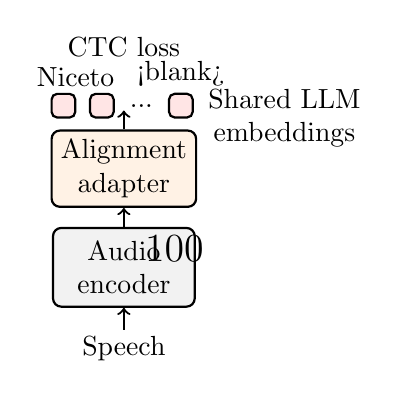
\begin{tikzpicture} [scale=0.8]
        \node(ae) at (0,0) [rectangle, draw=black, fill=gray!10, rounded corners=3pt, thick, minimum width=1.8cm,minimum height=1cm,align=center] {Audio\\encoder};
        \node(freeze) at ([xshift=0.8cm,yshift=0.3cm]ae.center) [rectangle, align=center] {\Large{\ding{100}}};
        \node(fb) at ([yshift=-0.3cm]ae.south) [rectangle, align=center,anchor=north] {Speech};
        \node(aa) at ([yshift=0.3cm]ae.north) [rectangle, draw=black, fill=orange!10, rounded corners=3pt, thick, minimum width=1.8cm,minimum height=0.5cm,align=center,anchor=south] {Alignment\\adapter};
        
        \node(f1) at ([yshift=1.0cm]aa.west) [rectangle, draw=black, fill=red!10, rounded corners=2pt, thick, minimum width=0.3cm, minimum height=0.3cm,align=center,anchor=west] {};
        \node(f2) at ([xshift=0.2cm]f1.east) [rectangle, draw=black, fill=red!10, rounded corners=2pt, thick, minimum width=0.3cm, minimum height=0.3cm,align=center,anchor=west] {};
        \node(f3) at ([xshift=0.075cm]f2.east) [rectangle, draw=white,  thick, align=center,anchor=west] {...};
        \node(f4) at ([xshift=0.075cm]f3.east) [rectangle, draw=black, fill=red!10, rounded corners=2pt, thick, minimum width=0.3cm, minimum height=0.3cm,align=center,anchor=west] {};
        \node(t1) at ([yshift=-0.05cm]f1.north) [rectangle, align=center,anchor=south] {Nice};
        \node(t2) at ([yshift=-0.05cm]f2.north) [rectangle, align=center,anchor=south] {to};
        \node(t4) at ([yshift=-0.05cm]f4.north) [rectangle, align=center,anchor=south] {<blank>};
        \node(se) at ([xshift=0.075cm,yshift=-0.2cm]f4.east) [rectangle, align=center,anchor=west] {Shared LLM\\embeddings};
        \node(ctc) at ([yshift=1.0cm]aa.north) [rectangle, rounded corners=3pt, thick, align=center,anchor=south] {CTC loss};

        
        \draw[->,thick]([yshift=-0.05cm]fb.north)--(ae.south);
        \draw[->,thick](ae.north)--(aa.south);
        \draw[->,thick](aa.north)--([yshift=0.3cm]aa.north);

        
      \end{tikzpicture}
    \end{minipage}
    }
    \subfigure[Shrinking stage]{
    \begin{minipage}[t]{0.45\linewidth}
    \centering
    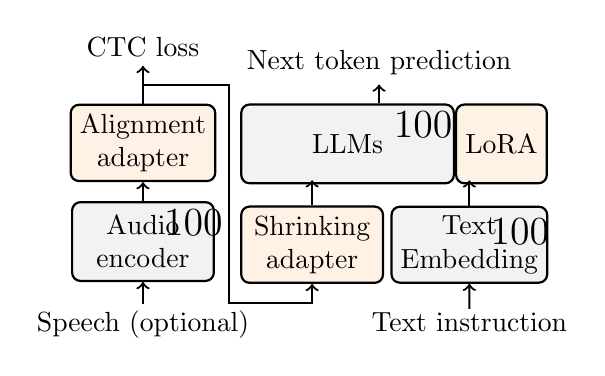
\begin{tikzpicture} [scale=0.8]
        \node(ae) at (0,0) [rectangle, draw=black, fill=gray!10, rounded corners=3pt, thick, minimum width=1.8cm,minimum height=1cm,align=center] {Audio\\encoder};
        \node(freeze) at ([xshift=0.8cm,yshift=0.3cm]ae.center) [rectangle, align=center] {\Large{\ding{100}}};
        \node(fb) at ([yshift=-0.3cm]ae.south) [rectangle, align=center,anchor=north] {Speech (optional)};
        \node(aa) at ([yshift=0.3cm]ae.north) [rectangle, draw=black, fill=orange!10, rounded corners=3pt, thick, minimum width=1.8cm,minimum height=0.5cm,align=center,anchor=south] {Alignment\\adapter};
        \node(ctc) at ([yshift=0.6cm]aa.north) [rectangle,align=center,anchor=south] {CTC loss};
        \node(sa) at ([xshift=0.4cm,yshift=-0.05cm]ae.east) [rectangle, draw=black, fill=orange!10, rounded corners=3pt, thick, minimum width=1.8cm,minimum height=0.5cm,align=center,anchor=west] {Shrinking\\adapter};
        \node(llm) at ([yshift=1.6cm]sa.west) [rectangle, draw=black, fill=gray!10, rounded corners=3pt, thick, minimum width=2.7cm,minimum height=1.0cm,align=center,anchor=west] {LLMs};
        \node(lora) at (llm.east) [rectangle, draw=black, fill=orange!10, rounded corners=3pt, thick, minimum width=1.0cm,minimum height=1.0cm,align=center,anchor=west] {LoRA};
        \node(te) at ([xshift=0.1cm]sa.east) [rectangle, draw=black, fill=gray!10, rounded corners=3pt, thick, minimum width=1.8cm,minimum height=0.5cm,align=center,anchor=west] {Text\\Embedding};
        \node(freeze3) at ([xshift=0.8cm,yshift=0.2cm]te.center) [rectangle, align=center] {\Large{\ding{100}}};
        \node(ti) at ([yshift=-0.3cm]te.south) [rectangle, align=center,anchor=north] {Text instruction};
        \node(freeze2) at ([xshift=1.2cm,yshift=0.3cm]llm.center) [rectangle, align=center] {\Large{\ding{100}}};
        \node(loss) at ([xshift=0.5cm, yshift=0.3cm]llm.north) [rectangle, align=center,anchor=south] {Next token prediction};

        
        \draw[->,thick]([yshift=-0.05cm]fb.north)--(ae.south);
        \draw[->,thick](ae.north)--(aa.south);
        \draw[->,thick](aa.north)--(ctc.south);
        \draw[->,thick](sa.north)--([yshift=0.4cm]sa.north);
        \draw[->,thick](te.north)--([yshift=0.4cm]te.north);
        \draw[->,thick]([yshift=-0.3cm]loss.south)--(loss.south);
        \draw[->,thick]([yshift=-0.1cm]ti.north)--(te.south);

        \draw[->,thick](aa.north)--([yshift=0.3cm]aa.north)--([xshift=0.2cm, yshift=0.3cm]aa.north -| aa.east)--([xshift=0.2cm, yshift=-0.3cm]sa.south -| aa.east)--([yshift=-0.3cm]sa.south)--(sa.south);
      \end{tikzpicture}
    \end{minipage}
    }
    \subfigure[SFT stage]{
    \begin{minipage}[t]{0.20\linewidth}
    \centering
    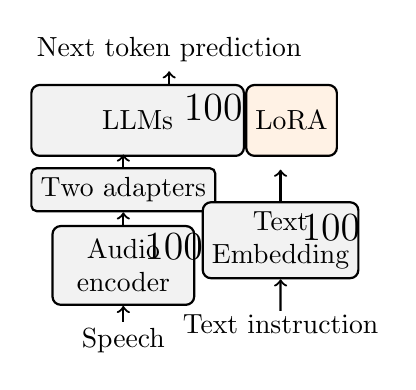
\begin{tikzpicture} [scale=0.8]
        \node(ae) at (0,0) [rectangle, draw=black, fill=gray!10, rounded corners=3pt, thick, minimum width=1.8cm,minimum height=1cm,align=center] {Audio\\encoder};
        \node(freeze) at ([xshift=0.8cm,yshift=0.3cm]ae.center) [rectangle, align=center] {\Large{\ding{100}}};
        \node(fb) at ([yshift=-0.2cm]ae.south) [rectangle, align=center,anchor=north] {Speech};
        \node(aa) at ([yshift=0.2cm]ae.north) [rectangle, draw=black, fill=gray!10, rounded corners=2pt, thick, minimum width=1.8cm,minimum height=0.5cm,align=center,anchor=south] {Two adapters};
        
        \node(llm) at ([yshift=1.1cm]aa.west) [rectangle, draw=black, fill=gray!10, rounded corners=3pt, thick, minimum width=2.7cm,minimum height=0.9cm,align=center,anchor=west] {LLMs};
        \node(lora) at (llm.east) [rectangle, draw=black, fill=orange!10, rounded corners=3pt, thick, minimum width=0.9cm,minimum height=0.9cm,align=center,anchor=west] {LoRA};
        \node(te) at ([xshift=0.1cm,yshift=0.4cm]ae.east) [rectangle, draw=black, fill=gray!10, rounded corners=3pt, thick, minimum width=1.8cm,minimum height=0.5cm,align=center,anchor=west] {Text\\Embedding};
        \node(freeze3) at ([xshift=0.8cm,yshift=0.2cm]te.center) [rectangle, align=center] {\Large{\ding{100}}};
        \node(ti) at ([yshift=-0.4cm]te.south) [rectangle, align=center,anchor=north] {Text instruction};
        \node(freeze2) at ([xshift=1.2cm,yshift=0.2cm]llm.center) [rectangle, align=center] {\Large{\ding{100}}};
        \node(loss) at ([xshift=0.5cm, yshift=0.2cm]llm.north) [rectangle, align=center,anchor=south] {Next token prediction};
       
        \draw[->,thick]([yshift=-0.05cm]fb.north)--(ae.south);
        \draw[->,thick](ae.north)--(aa.south);
        \draw[->,thick](aa.north)--([yshift=0.2cm]aa.north);
        \draw[->,thick](te.north)--([yshift=0.5cm]te.north);
        \draw[->,thick]([yshift=-0.2cm]loss.south)--(loss.south);
        \draw[->,thick]([yshift=-0.1cm]ti.north)--(te.south);
        
      \end{tikzpicture}
    \end{minipage}
    }
      \caption{Training progress of Soundwave. The gray modules are frozen while the orange modules are updated.}
      \label{architecture}
  \end{figure*}

  


\section{Implementation and Evaluation}
\label{sec:evaluation}

We prototype our proposal into a tool \toolName, using approximately 5K lines of OCaml (for the program analysis) and 5K lines of Python code (for the repair). 
In particular, we employ Z3~\cite{DBLP:conf/tacas/MouraB08} as the SMT solver, clingo~\cite{DBLP:books/sp/Lifschitz19} as the ASP solver, and Souffle~\cite{scholz2016fast} as the Datalog engine. %, respectively.
To show the effectiveness, 
we design the experimental evaluation to answer the 
following research questions (RQ):
(Experiments ran on a server with an Intel® Xeon® Platinum 8468V, 504GB RAM, and 192 cores. All the dataset are publicly available from \cite{zenodo_benchmark})

\begin{itemize}[align=left, leftmargin=*,labelindent=0pt]
\item \textbf{RQ1:} How effective is \toolName in verifying CTL properties for relatively small but complex programs, compared to the state-of-the-art tool  \function~\cite{DBLP:conf/sas/UrbanU018}?


\item \textbf{RQ2:} What is the effectiveness of \toolName in detecting real-world bugs, which can be encoded using both CTL and linear temporal logic (LTL), such as non-termination gathered from GitHub \cite{DBLP:conf/sigsoft/ShiXLZCL22} and unresponsive behaviours in protocols  \cite{DBLP:conf/icse/MengDLBR22}, compared with \ultimate~\cite{DBLP:conf/cav/DietschHLP15}?

\item \textbf{RQ3:} How effective is \toolName in repairing CTL violations identified in RQ1 and RQ2? which has not been achieved by any existing tools. 


 

\end{itemize}



% \begin{itemize}[align=left, leftmargin=*,labelindent=0pt]
% \item \textbf{RQ1:} What is the effectiveness of \toolName in verifying CTL properties in a set of relatively small yet challenging programs, compared to the state-of-the-art tools, T2~\cite{DBLP:conf/fmcad/CookKP14},  \function~\cite{DBLP:conf/sas/UrbanU018}, and \ultimate~\cite{DBLP:conf/cav/DietschHLP15}?


% \item \textbf{RQ2:} What is the effectiveness of \toolName in finding  real-world bugs, which can be encoded using CTL properties, such as non-termination 
% gathered from GitHub \cite{DBLP:conf/sigsoft/ShiXLZCL22} and unresponsive behaviours in protocol implementations \cite{DBLP:conf/icse/MengDLBR22}?

% \item \textbf{RQ3:} What is the effectiveness of \toolName in repairing CTL bugs from RQ1--2?

% \end{itemize}

%The benchmark programs are from various sources. More specifically, termination bugs from real-world projects \cite{DBLP:conf/sigsoft/ShiXLZCL22} and CTL analysis \cite{DBLP:conf/fmcad/CookKP14} \cite{DBLP:conf/sas/UrbanU018}, and temporal bugs in real-world protocol implementations \cite{DBLP:conf/icse/MengDLBR22}. 



% \ly{are termination bugs ok? Do we need to add new CTL bugs?}
\subsection{RQ1: Verifying CTL Properties}

% Please add the following required packages to your document preamble:
%  \Xhline{1.5\arrayrulewidth}

\hide{\begin{figure}[!h]
\vspace{-8mm}
\begin{lstlisting}[xleftmargin=0.2em,numbersep=6pt,basicstyle=\footnotesize\ttfamily]
(*@\textcolor{mGray}{//$EF(\m{resp}{\geq}5)$}@*)
int c = *; int resp = 0;
int curr_serv = 5; 
while (curr_serv > 0){ 
 if (*) {  
   c--; 
   curr_serv--;
   resp++;} 
 else if (c<curr_serv){
   curr_serv--; }}
\end{lstlisting} 
\vspace{-2mm}
\caption{A possibly terminating loop} 
\label{fig:terminating_loop}
\vspace{-2mm}
\end{figure}}


%loses precision due to a \emph{dual widening} \cite{DBLP:conf/tacas/CourantU17}, and 

The programs listed in \tabref{tab:comparewithFuntionT2} were obtained from the evaluation benchmark of \function, which includes a total of 83 test cases across over 2,000 lines of code. We categorize these test cases into six groups, labeled according to the types of CTL properties. 
These programs are short but challenging, as they often involve complex loops or require a more precise analysis of the target properties. The \function tends to be conservative, often leading it to return ``unknown" results, resulting in an accuracy rate of 27.7\%. In contrast, \toolName demonstrates advantages with improved accuracy, particularly in \ourToolSmallBenchmark. 
%achieved by the novel loop summaries. 
The failure cases faced by \toolName highlight our limitations when loop guards are not explicitly defined or when LRFs are inadequate to prove termination. 
Although both \function and \toolName struggle to obtain meaningful invariances for infinite loops, the benefits of our loop summaries become more apparent when proving properties related to termination, such as reachability and responsiveness.  




\begin{table}[!t]
\vspace{1.5mm}
\caption{Detecting real-world CTL bugs.}
\normalsize
\label{tab:comparewithCook}
\renewcommand{\arraystretch}{0.95}
\setlength{\tabcolsep}{4pt}  
\begin{tabular}{c|l|c|cc|cc}
\Xhline{1.5\arrayrulewidth}
\multicolumn{1}{l|}{\multirow{2}{*}{\textbf{}}} & \multirow{2}{*}{\textbf{Program}}        & \multirow{2}{*}{\textbf{LoC}} & \multicolumn{2}{c|}{\textbf{\ultimateshort}}   & \multicolumn{2}{c}{\textbf{\toolName}}             \\ \cline{4-7} 
  \multicolumn{1}{l|}{}                           &                                          &                               & \multicolumn{1}{c|}{\textbf{Res.}} & \textbf{Time} & \multicolumn{1}{c|}{\textbf{Res.}} & \textbf{Time} \\ \hline
  1 \xmark                                      & \multirow{2}{*}{\makecell[l]{libvncserver\\(c311535)}}   & 25                            & \multicolumn{1}{c|}{\xmark}      & 2.845         & \multicolumn{1}{c|}{\xmark}      & 0.855         \\  
  1 \cmark                                      &                                          & 27                            & \multicolumn{1}{c|}{\cmark}      & 3.743         & \multicolumn{1}{c|}{\cmark}      & 0.476         \\ \hline
  2 \xmark                                      & \multirow{2}{*}{\makecell[l]{Ffmpeg\\(a6cba06)}}         & 40                            & \multicolumn{1}{c|}{\xmark}      & 15.254        & \multicolumn{1}{c|}{\xmark}      & 0.606         \\  
  2 \cmark                                      &                                          & 44                            & \multicolumn{1}{c|}{\cmark}      & 40.176        & \multicolumn{1}{c|}{\cmark}      & 0.397         \\ \hline
  3 \xmark                                      & \multirow{2}{*}{\makecell[l]{cmus\\(d5396e4)}}           & 87                            & \multicolumn{1}{c|}{\xmark}      & 6.904         & \multicolumn{1}{c|}{\xmark}      & 0.579         \\  
  3 \cmark                                      &                                          & 86                            & \multicolumn{1}{c|}{\cmark}      & 33.572        & \multicolumn{1}{c|}{\cmark}      & 0.986         \\ \hline
  4 \xmark                                      & \multirow{2}{*}{\makecell[l]{e2fsprogs\\(caa6003)}}      & 58                            & \multicolumn{1}{c|}{\xmark}      & 5.952         & \multicolumn{1}{c|}{\xmark}      & 0.923         \\  
  4 \cmark                                      &                                          & 63                            & \multicolumn{1}{c|}{\cmark}      & 4.533         & \multicolumn{1}{c|}{\cmark}      & 0.842         \\ \hline
  5 \xmark                                      & \multirow{2}{*}{\makecell[l]{csound-an...\\(7a611ab)}} & 43                            & \multicolumn{1}{c|}{\xmark}      & 3.654         & \multicolumn{1}{c|}{\xmark}      & 0.782         \\  
  5 \cmark                                      &                                          & 45                            & \multicolumn{1}{c|}{TO}          & -             & \multicolumn{1}{c|}{\cmark}      & 0.648         \\ \hline
  6 \xmark                                      & \multirow{2}{*}{\makecell[l]{fontconfig\\(fa741cd)}}     & 25                            & \multicolumn{1}{c|}{\xmark}      & 3.856         & \multicolumn{1}{c|}{\xmark}      & 0.769         \\  
  6 \cmark                                      &                                          & 25                            & \multicolumn{1}{c|}{Error}       & -             & \multicolumn{1}{c|}{\cmark}      & 0.651         \\ \hline
  7 \xmark                                      & \multirow{2}{*}{\makecell[l]{asterisk\\(3322180)}}       & 22                            & \multicolumn{1}{c|}{\unk}        & 12.687        & \multicolumn{1}{c|}{\unk}        & 0.196         \\  
  7 \cmark                                      &                                          & 25                            & \multicolumn{1}{c|}{\unk}        & 11.325        & \multicolumn{1}{c|}{\unk}        & 0.34          \\ \hline
  8 \xmark                                      & \multirow{2}{*}{\makecell[l]{dpdk\\(cd64eeac)}}          & 45                            & \multicolumn{1}{c|}{\xmark}      & 3.712         & \multicolumn{1}{c|}{\xmark}      & 0.447         \\  
  8 \cmark                                      &                                          & 45                            & \multicolumn{1}{c|}{\cmark}      & 2.97          & \multicolumn{1}{c|}{\unk}        & 0.481         \\ \hline
  9 \xmark                                      & \multirow{2}{*}{\makecell[l]{xorg-server\\(930b9a06)}}   & 19                            & \multicolumn{1}{c|}{\xmark}      & 3.111         & \multicolumn{1}{c|}{\xmark}      & 0.581         \\  
  9 \cmark                                      &                                          & 20                            & \multicolumn{1}{c|}{\cmark}      & 3.101         & \multicolumn{1}{c|}{\cmark}      & 0.409         \\ \hline
  10 \xmark                                      & \multirow{2}{*}{\makecell[l]{pure-ftpd\\(37ad222)}}      & 42                            & \multicolumn{1}{c|}{\cmark}      & 2.555         & \multicolumn{1}{c|}{\xmark}      & 0.933         \\  
  10 \cmark                                      &                                          & 49                            & \multicolumn{1}{c|}{\cmark}        & 2.286         & \multicolumn{1}{c|}{\cmark}      & 0.383         \\ \hline
  11 \xmark  & \multirow{2}{*}{\makecell[l]{live555$_a$\\(181126)}} & 34  & \multicolumn{1}{c|}{\cmark} &  2.715         & \multicolumn{1}{c|}{\xmark}    & 0.513   \\  
  11 \cmark  &     &   37    & \multicolumn{1}{c|}{\cmark} &  2.837         & \multicolumn{1}{c|}{\cmark}      & 0.341 \\ \hline
  12 \xmark  & \multirow{2}{*}{\makecell[l]{openssl\\(b8d2439)}} & 88  & \multicolumn{1}{c|}{\xmark} &  4.15          & \multicolumn{1}{c|}{\xmark}    & 0.78   \\
  12 \cmark  &     &  88     & \multicolumn{1}{c|}{\cmark} &  3.809         & \multicolumn{1}{c|}{\cmark}      & 0.99 \\ \hline
  13 \xmark  & \multirow{2}{*}{\makecell[l]{live555$_b$\\(131205)}} & 83  & \multicolumn{1}{c|}{\xmark} & 2.838         & \multicolumn{1}{c|}{\xmark}    & 0.602     \\  
  13 \cmark  &    &   84     & \multicolumn{1}{c|}{\cmark} &  2.393         & \multicolumn{1}{c|}{\cmark}      & 0.565 \\ \Xhline{1.5\arrayrulewidth}
                                                   & {\bf{Total}}                                  & 1249  & \multicolumn{1}{c|}{\bestBaseLineReal}          & $>$180       & \multicolumn{1}{c|}{\ourToolRealBenchmark}              & 16.01        \\ \Xhline{1.5\arrayrulewidth}
  \end{tabular}
  \end{table}

\subsection{RQ2: CTL Analysis on  Real-world Projects}




Programs in \tabref{tab:comparewithCook} are from real-world repositories, each associated with a Git commit number where developers identify and fix the bug manually. 
In particular, the property used for programs 1-9 (drawn from \cite{DBLP:conf/sigsoft/ShiXLZCL22}) is  \code{AF(Exit())}, capturing non-termination bugs. The properties used for programs 10-13 (drawn from \cite{DBLP:conf/icse/MengDLBR22}) are of the form \code{AG(\phi_1{\rightarrow}AF(\phi_2))}, capturing unresponsive behaviours from the protocol implementation. 
We extracted the main segments of these real-world bugs into smaller programs (under 100 LoC each), preserving features like data structures and pointer arithmetic. Our evaluation includes both buggy (\eg 1\,\xmark) and developer-fixed (\eg 1\,\cmark) versions.
After converting the CTL properties to LTL formulas, we compared our tool with the latest release of UltimateLTL (v0.2.4), a regular participant in SV-COMP \cite{svcomp} with competitive performance. 
Both tools demonstrate high accuracy in bug detection, while \ultimateshort often requires longer processing time. 
This experiment indicates that LRFs can effectively handle commonly seen real-world loops, and \toolName performs a more lightweight summary computation without compromising accuracy. 



%Following the convention in \cite{DBLP:conf/sigsoft/ShiXLZCL22}, t
%Prior works \cite{DBLP:conf/sigsoft/ShiXLZCL22} gathered such examples by extracting 
%\toolName successfully identifies the majority of buggy and correct programs, with the exception of programs 7 and 8. 







{
\begin{table*}[!h]
  \centering
\caption{\label{tab:repair_benchmark}
{Experimental results for repairing CTL bugs. Time spent by the ASP solver is separately recorded. 
}
}
\small
\renewcommand{\arraystretch}{0.95}
  \setlength{\tabcolsep}{9pt}
\begin{tabular}{l|c|c|c|c|c|c|c|c}
  \Xhline{1.5\arrayrulewidth}
  \multicolumn{1}{c|}{\multirow{2}{*}{\textbf{Program}}} & \multicolumn{1}{c|}{\multirow{2}{*}{\shortstack{\textbf{LoC}\\\textbf{(Datalog)}}}} & \multicolumn{3}{c|}{\textbf{Configuration}}                                 & \multicolumn{1}{c|}{\multirow{2}{*}{\textbf{Fixed}}} & \multicolumn{1}{c|}{\multirow{2}{*}{\textbf{\#Patch}}} & \multicolumn{1}{c|}{\multirow{2}{*}{\textbf{ASP(s)}}} & \multirow{2}{*}{\textbf{Total(s)}} \\ \cline{3-5}

  \multicolumn{1}{c|}{}                                  & \multicolumn{1}{c|}{}                              & \multicolumn{1}{c|}{\textbf{Symbols}} & \multicolumn{1}{c|}{\textbf{Facts}} & \multicolumn{1}{c|}{\textbf{Template}} & \multicolumn{1}{c|}{} & \multicolumn{1}{c|}{} & \multicolumn{1}{c|}{}  &                                      \\ \hline

AF\_yEQ5 (\figref{fig:first_Example})                                           & 115                           & 3+0                   & 0+1                & Add                & \cmark     & 1                   & 0.979                              & 1.593                                \\
test\_until.c                                         & 101                            & 0+3                   & 1+0                & Delete                & \cmark     & 1                   & 0.023                              & 0.498                                \\
next.c                                                & 87                            & 0+4                   & 1+0                & Delete                & \cmark     & 1                   & 0.023                              & 0.472                                \\
libvncserver                                          & 118                            & 0+6                   & 1+0                & Delete                & \cmark     & 3                   & 0.049                              & 1.081                                \\
Ffmpeg                                                & 227                           & 0+12                  & 1+0                & Delete                & \cmark     & 4                   & 13.113                              & 13.335                                \\
cmus                                                  & 145                           & 0+12                  & 1+0                & Delete                & \cmark     & 4                   & 0.098                              & 2.052                                \\
e2fsprogs                                             & 109                           & 0+8                   & 1+0                & Delete                & \cmark     & 2                   & 0.075                              & 1.515                                \\
csound-android                                        & 183                           & 0+8                   & 1+0                & Delete                & \cmark     & 4                   & 0.076                              & 1.613                                \\
fontconfig                                            & 190                           & 0+11                  & 1+0                & Delete                & \cmark     & 6                   & 0.098                              & 2.507                                \\
dpdk                                                  & 196                           & 0+12                  & 1+0                & Delete                & \cmark     & 1                   & 0.091                              & 2.006                                \\
xorg-server                                           & 118                            & 0+2                   & 1+0                & Delete                & \cmark     & 2                   & 0.026                              & 0.605                                \\
pure-ftpd                                             & 258                           & 0+21                  & 1+0                & Delete                & \cmark     & 2                   & 0.069                              & 3.590                               \\
live$_a$                                              & 112                            & 3+4                   & 1+1                & Update                & \cmark     & 1                   & 0.552                              & 0.816                                \\
openssl                                               & 315                           & 1+0                   & 0+1                & Add.                & \cmark     & 1                   & 1.188                              & 2.277                                \\
live$_b$                                              & 217                           & 1+0                   & 0+1                & Add                & \cmark     & 1                   & 0.977                              & 1.494                                 \\
  \Xhline{1.5\arrayrulewidth}
\textbf{Total}                                                 & 2491                          &                       &                    &                   &           &                     & 17.437                              & 35.454                               \\ 
  \Xhline{1.5\arrayrulewidth}           
\end{tabular}

\vspace{-2mm}
\end{table*}
}


\subsection{RQ3: Repairing CTL Property Violations} 


\tabref{tab:repair_benchmark} gathers all the program instances (from \tabref{tab:comparewithFuntionT2} and \tabref{tab:comparewithCook}) that violate their specified CTL properties and are sent to \toolName for repair.   
The \textbf{Symbols} column records the number of symbolic constants + symbolic signs, while the \textbf{Facts} column records the number of facts allowed to be removed + added. 
We gradually increase the number of symbols and the maximum number of facts that can be added or deleted. 
The \textbf{Configuration} column shows the first successful configuration that led to finding patches, and we record the total searching time till reaching such configurations. 
We configure \toolName to apply three atomic templates in a breadth-first manner with a depth limit of 1, \ie, \tabref{tab:repair_benchmark} records the patch result after one iteration of the repair. 
The templates are applied sequentially in the order: delete, update, and add. The repair process stops when a correct patch is found or when all three templates have been attempted. 
%without success. 
% Because of this configuration, \toolName only finds one patch for Program 1 (AF\_yEQ5). 
% The patch inserting \plaincode{if (i>10||x==y) \{y=5; return;\}} mentioned in \figref{fig:Patched-program} cannot be found in current configuration, as it requires deleting facts then adding new facts on the updated program.
% The `Configuration' column in \tabref{tab:repair_benchmark} shows the number of symbolic constants and signs, the number of facts allowed to be removed and added, and the template used when a patch is found.

Due to the current configuration, \toolName only finds patch (b) for Program 1 (AF\_yEQ5), while the patch (a) shown in \figref{fig:Patched-program} can be obtained by allowing two iterations of the repair: the first iteration adds the conditional than a second iteration to add a new assignment on the updated program. 
Non-termination bugs are resolved within a single iteration by adding a conditional statement that provides an earlier exit. 
For instance, \figref{fig:term-Patched-program} illustrates the main logic of 1\,\xmark, which enters an infinite loop when \code{\m{linesToRead}{\leq}0}. 
\toolName successfully 
provides a fix that prevents \code{\m{linesToRead}{\leq}0} from occurring before entering the loop. Note that such patches are more desirable which fix the non-termination bug without dropping the loops completely. 
%much like the example shown in  \figref{fig:term-Patched-program}. At the same time, 
Unresponsive bugs involve adding more function calls or assignment modifications. 
%Most repairs were completed within seconds. 

On average, the time taken to solve ASP accounts for 49.2\% (17.437/35.454) of the total repair time. We also keep track of the number of patches that successfully eliminate the CTL violations. More than one patch is available for non-termination bugs, as some patches exit the entire program without entering the loop. 
While all the patches listed are valid, those that intend to cut off the main program logic can be excluded based on the minimum change criteria. 
After a manual inspection of each buggy program shown in \tabref{tab:repair_benchmark}, we confirmed that at least one generated patch is semantically equivalent to the fix provided by the developer. 
As the first tool to achieve automated repair of CTL violations, \toolName successfully resolves all reported bugs. 



\begin{figure}[!t]
\begin{lstlisting}[xleftmargin=6em,numbersep=6pt,basicstyle=\footnotesize\ttfamily]
void main(){ //AF(Exit())
  int lines ToRead = *;
  int h = *;
  (*@\repaircode{if ( linesToRead <= 0 )  return;}@*)
  while(h>0){
    if(linesToRead>h)  
        linesToRead=h; 
    h-=linesToRead;} 
  return;}
\end{lstlisting}
\caption{Fixing a Possible Hang Found in libvncserver \cite{LibVNCClient}}
\label{fig:term-Patched-program}
\end{figure}


\section{Analysis}
\label{sec:analysis}
In the following sections, we will analyze European type approval regulation\footnote{Strictly speaking, the German enabling act (AFGBV) does not regulate type-approval, but how test \& operating permits are issued for SAE-Level-4 systems. Type-approval regulation for SAE-Level-3 systems follows UN Regulation No. 157 (UN-ECE-ALKS) \parencite{un157}.} regarding the underlying notions of ``safety'' and ``risk''.
We will classify these notions according to their absolute or relative character, underlying risk sources, or underlying concepts of harm.

\subsection{Classification of Safety Notions}
\label{sec:safety-notions}
We will refer to \emph{absolute} notions of safety as conceptualizations that assume the complete absence of any kind of risk.
Opposed to this, \emph{relative} notions of safety are based on a conceptualization that specifically includes risk acceptance criteria, e.g., in terms of ``tolerable'' risk or ``sufficient'' safety.

For classifying notions of safety by their underlying risk (or rather ``hazard'') sources, and different concepts of harm, \Cref{fig:hazard-sources} provides an overview of our reasoning, which is closely in line with the argumentation provided by Waymo in \parencite{favaro2023}.
We prefer ``hazard sources'' over ``risk sources'', as a risk must always be related to a \emph{cause} or \emph{source of harm} (i.e., a hazard \parencite[p.~1, def. 3.2]{iso51}).
Without a concrete (scenario) context that the system is operating in, a hazard is \emph{latent}: E.g., when operating in public traffic, there is a fundamental possibility that a \emph{collision with a pedestrian} leads to (physical) harm for that pedestrian. 
However, only if an automated vehicle shows (potentially) hazardous behavior (e.g., not decelerating properly) \emph{and} is located near a pedestrian (context), the hazard is instantiated and leads to a hazardous event.
\begin{figure*}
    \includeimg[width=.9\textwidth]{hazard-sources0.pdf}
    \caption{Graphical summary of a taxonomy of risk related to automated vehicles, extended based on ISO 21448 (\parencite{iso21448}) and \parencite{favaro2023}. Top: Causal chain from hazard sources to actual harm; bottom: summary of the individual elements' contributions to a resulting risk. Graphic translated from \parencite{nolte2024} \label{fig:hazard-sources}}
\end{figure*}
If the hazardous event cannot be mitigated or controlled, we see a loss event in which the pedestrian's health is harmed.
Note that this hypothetical chain of events is summarized in the definition of risk:
The probability of occurrence of harm is determined by a) the frequency with which hazard sources manifest, b) the time for which the system operates in a context that exposes the possibility of harm, and c) by the probability with which a hazardous event can be controlled.
A risk can then be determined as a function of the probability of harm and the severity of the harm potentially inflicted on the pedestrian.

In the following, we will apply this general model to introduce different types of hazard sources and also different types of harm.
\cref{fig:hazard-sources} shows two distinct hazard sources, i.e., functional insufficiencies and E/E-failures that can lead to hazardous behavior.
ISO~21488 \parencite{iso21448} defines functional insufficiencies as insufficiencies that stem from an incomplete or faulty system specification (specification insufficiencies).
In addition, the standard considers insufficiencies that stem from insufficient technical capability to operate inside the targeted Operational Design Domain (performance insufficiencies).
Functional insufficiencies are related to the ``Safety of the Intended Functionality (SOTIF)'' (according to ISO~21448), ``Behavioral Safety'' (according to Waymo \parencite{waymo2018}), or ``Operational Safety'' (according to UN Regulation No. 157 \parencite{un157}).
E/E-Failures are related to classic functional safety and are covered exhaustively by ISO~26262 \parencite{iso2018}.
Additional hazard sources can, e.g., be related to malicious security attacks (ISO~21434), or even to mechanical failures that should be covered (in the US) in the Federal Motor Vehicle Safety Standards (FMVSS).

For the classification of notions of safety by the related harm, in \parencite{salem2024, nolte2024}, we take a different approach compared to \parencite{koopman2024}:
We extend the concept of harm to the violation of stakeholder \emph{values}, where values are considered to be a ``standard of varying importance among other such standards that, when combined, form a value pattern that reduces complexity for stakeholders [\ldots] [and] determines situational actions [\ldots].'' \parencite{albert2008}
In this sense, values are profound, personal determinants for individual or collective behavior.
The notion of values being organized in a weighted value pattern shows that values can be ranked according to importance.
For automated vehicles, \emph{physical wellbeing} and \emph{mobility} can, e.g., be considered values which need to be balanced to achieve societal acceptance, in line with the discussion of required tradeoffs in \cref{sec:terminology}.
For the analysis of the following regulatory frameworks, we will evaluate if the given safety or risk notions allow tradeoffs regarding underlying stakeholder values. 

\subsection{UN Regulation No. 157 \& European Implementing Regulation (EU) 2022/1426}
\label{sec:enabling-act}
UN Regulation No. 157 \parencite{un157} and the European Implementing Regulation 2022/1426 \parencite{eu1426} provide type approval regulation for automated vehicles equipped with SAE-Level-3 (UN Reg. 157) and Level 4 (EU 2022/1426) systems on an international (UN Reg. 157) and European (EU 2022/1426) level.

Generally, EU type approval considers UN ECE regulations mandatory for its member states ((EU) 2018/858, \parencite{eu858}), while the EU largely forgoes implementing EU-specific type approval rules, it maintains the right to alter or to amend UN ECE regulation \parencite{eu858}.

In this respect, the terminology and conceptualizations in the EU Implementing Act closely follow those in UN Reg. No. 157.
The EU Implementing Act gives a clear reference to UN Reg. No. 157 \parencite[][Preamble,  Paragraph 1]{eu1426}.
Hence, the documents can be assessed in parallel.
Differences will be pointed out as necessary.

Both acts are written in rather technical language, including the formulation of technical requirements (e.g., regarding deceleration values or speeds in certain scenarios).
While providing exhaustive definitions and terminology, neither of both documents provide an actual definition of risk or safety.
The definition of ``unreasonable'' risk in both documents does not define risk, but only what is considered \emph{unreasonable}. It states that the ``overall level of risk for [the driver, (only in UN Reg. 157)] vehicle occupants and other road users which is increased compared to a competently and carefully driven manual vehicle.''
The pertaining notions of safety and risk can hence only be derived from the context in which they are used.

\subsubsection{Absolute vs. Relative Notions of Safety}
In line with the technical detail provided in the acts, both clearly imply a \emph{relative} notion of safety and refer to the absence of \emph{unreasonable} risk throughout, which is typical for technical safety definitions.

Both acts require sufficient proof and documentation that the to-be-approved automated driving systems are ``free of unreasonable safety risks to vehicle occupants and other road users'' for type approval.\footnote{As it targets SAE-Level-3 systems, UN Reg. 157 also refers to the driver, where applicable.}
In this respect, both acts demand that the manufacturers perform verification and validation activities for performance requirements that include ``[\ldots] the conclusion that the system is designed in such a way that it is free from unreasonable risks [\ldots]''.
Additionally, \emph{risk minimization} is a recurring theme when it comes to the definition of Minimum Risk Maneuvers (MRM).

Finally, supporting the relative notions of safety and risk, UN Reg. 157 introduces the concept of ``reasonable foreseeable and preventable'' \parencite[Article 1, Clause 5.1.1.]{un157} collisions, which implies that a residual risk will remain with the introduction of automated vehicles.
\parencite[][Appendix 3, Clause 3.1.]{un157} explicitly states that only \emph{some} scenarios that are unpreventable for a competent human driver can actually be prevented by an automated driving system.
While this concept is not applied throughout the EU Implementing Act, both documents explicitly refer to \emph{residual} risks that are related to the operation of automated driving systems (\parencite[][Annex I, Clause 1]{un157}, \parencite[][Annex II, Clause 7.1.1.]{eu1426}).

\subsubsection{Hazard Sources}
Hazard sources that are explicitly differentiated in UN Reg. 157 and (EU) 2022/1426 are E/E-failures that are in scope of functional safety (ISO~26262) and functional insufficiencies that are in scope of behavioral (or ``operational'') safety (ISO~21448).
Both documents consistently differentiate both sources when formulating requirements.

While the acts share a common definition of ``operational'' safety (\parencite[][Article 2, def. 30.]{eu1426}, \parencite[][Annex 4, def. 2.15.]{un157}), the definitions for functional safety differ.
\parencite{un157} defines functional safety as the ``absence of unreasonable risk under the occurrence of hazards caused by a malfunctioning behaviour of electric/electronic systems [\ldots]'', \parencite{eu1426} drops the specification of ``electric/electronic systems'' from the definition.
When taken at face value, this definition would mean that functional safety included all possible hazard sources, regardless of their origin, which is a deviation from the otherwise precise usage of safety-related terminology.

\subsubsection{Harm Types}
As the acts lack explicit definitions of safety and risk, there is no consistent and explicit notion of different harm types that could be differentiated.

\parencite{un157} gives little hints regarding different considered harm types.
``The absence of unreasonable risk'' in terms of human driving performance could hence be related to any chosen performance metric that allows a comparison with a competent careful human driver including, e.g., accident statistics, statistics about rule violations, or changes in traffic flow.

In \parencite{eu1426}, ``safety'' is, implicitly, attributed to the absence of unreasonable risk to life and limb of humans.
This is supported by the performance requirements that are formulated:
\parencite[][Annex II, Clause 1.1.2. (d)]{eu1426} demands that an automated driving system can adapt the vehicle behavior in a way that it minimizes risk and prioritizes the protection of human life.

Both acts demand the adherence to traffic rules (\parencite[][Annex 2, Clause 1.3.]{eu1426}, \parencite[][Clause 5.1.2.]{un157}).
\parencite[][Annex II, Clause 1.1.2. (c)]{eu1426} also demands that an automated driving system shall adapt its behavior to surrounding traffic conditions, such as the current traffic flow.
With the relative notion of risk in both acts, the unspecific clear statement that there may be unpreventable accidents \parencite{un157}, and a demand of prioritization of human life in \parencite{eu1426}, both acts could be interpreted to allow developers to make tradeoffs as discussed in \cref{sec:terminology}.


\subsubsection{Conclusion}
To summarize, the UN Reg. 157 and the (EU) 2022/1426 both clearly support the technical notion of safety as the absence of unreasonable risk.
The notion is used consistently throughout both documents, providing a sufficiently clear terminology for the developers of automated vehicles.
Uncertainty remains when it comes to considered harm types: Both acts do not explicitly allow for broader notions of safety, in the sense of \parencite{koopman2024} or \parencite{salem2024}.
Finally, a minor weak spot can be seen in the definition of risk acceptance criteria: Both acts take the human driving performance as a baseline.
While (EU) 2022/1426 specifies that these criteria are specific to the systems' Operational Design Domain \parencite[][Annex II, Clause 7.1.1.]{eu1426}, the reference to the concrete Operational Design Domain is missing in UN Reg. 157.
Without a clearly defined notion of safety, however, it remains unclear, how aspects beyond net accident statistics (which are given as an example in \parencite[][Annex II, Clause 7.1.1.]{eu1426}), can be addressed practically, as demanded by \parencite{koopman2024}.

\subsection{German Regulation (StVG \& AFGBV)}
\label{sec:afgbv}
The German L3 (Automated Driving Act) and L4 (Act on Autonomous Driving) Acts from 2017 and 2021,\footnote{Formally, these are amendments to the German Road Traffic Act (StVG): 06/21/2017, BGBl. I p. 1648, 07/12/2021 BGBl. I p. 3108.} respectively, provide enabling regulation for the operation of SAE-Level-3 and 4 vehicles on German roads.
The German Implementing Regulation (\parencite{afgbv}, AFGBV) defines how this enabling regulation is to be implemented for granting testing permits for SAE-Level-3 and -4 and driving permits for SAE-Level-3 and -4 automated driving systems.\footnote{Note that these permits do not grant EU-wide type approval, but serve as a special solution for German roads only. At the same time, the AFGBV has the same scope as (EU) 2022/1426.}
With all three acts, Germany was the first country to regulate the approval of automated vehicles for a domestic market.
All acts are subject to (repeated) evaluation until the year 2030 regarding their impact on the development of automated driving technology.
An assessment of the German AFGBV and comparisons to (EU) 2022/1426 have been given in \cite{steininger2022} in German.

Just as for UN Reg. 157 and (EU) 2022/1426, neither the StVG nor the AFGBV provide a clear definition of ``safety'' or ``risk'' -- even though the "safety" of the road traffic is one major goal of the StVG and StVO.
Again, different implicit notions of both concepts can only be interpreted from the context of existing wording.
An additional complication that is related to the German language is that ``safety'' and ``security'' can both be addressed as ``Sicherheit'', adding another potential source of unclarity.
Literal Quotations in this section are our translations from the German act.

\subsubsection{Absolute vs. Relative Notions of Safety}
For assessing absolute vs. relative notions of safety in German regulation, it should be mentioned that the main goal of the German StVO is to ensure the ``safety and ease of traffic flow'' -- an already diametral goal that requires human drivers to make tradeoffs.\footnote{For human drivers, this also creates legal uncertainty which can sometimes only be settled in a-posteriori court cases.}
While UN and EU regulation clearly shows a relative notion of safety\footnote{And even the StVG contains sections that use wording such as ``best possible safety for vehicle occupants'' (§1d (4) StVG) and acknowledges that there are unavoidable hazards to human life (§1e (2) No. 2c)).}, the German AFGBV contains ambiguous statements in this respect:
Several paragraphs contain a demand for a hazard free operation of automated vehicles.
§4 (1) No. 4 AFGBV, e.g., states that ``the operation of vehicles with autonomous driving functions must neither negatively impact road traffic safety or traffic flow, nor endanger the life and limb of persons.''
Additionally, §6 (1) AFGBV states that the permits for testing and operation have to be revoked, if it becomes apparent that a ``negative impact on road traffic safety or traffic flow, or hazards to the life and limb of persons cannot be ruled out''.
The same wording is used for the approval of operational design domains regulated in §10 (1) No. 1.
A particularly misleading statement is made regarding the requirements for technical supervision instances which are regulated in §14 (3) AFGBV which states that an automated vehicle has to be  ``immediately removed from the public traffic space if a risk minimal state leads to hazards to road traffic safety or traffic flow''.
Considering the argumentation in \cref{sec:terminology}, that residual risks related to the operation of automated driving systems are inevitable, these are strong statements which, if taken at face value, technically prohibit the operation of automated vehicles.
It suggests an \emph{absolute} notion of safety that requires the complete absence of risk.  
The last statement above is particularly contradictory in itself, considering that a risk \emph{minimal} state always implies a residual risk.

In addition to these absolute safety notions, there are passages which suggest a relative notion of safety:
The approval for Operational Design Domains is coupled to the proof that the operation of an automated vehicle ``neither negatively impacts road traffic safety or traffic flow, nor significantly endangers the life and limb of persons beyond the general risk of an impact that is typical of local road traffic'' (§9 (2) No. 3 AFGBV).
The addition of a relative risk measure ``beyond the general risk of an impact'' provides a relaxation (cf. also \cite{steininger2022}, who criticizes the aforementioned absolute safety notion) that also yields an implicit acceptance criterion (\emph{statistically as good as} human drivers) similar to the requirements stated in UN Reg. 157 and (EU) 2022/1426.

Additional hints for a relative notion of safety can be found in Annex 1, Part 1, No. 1.1 and Annex 1, Part 2, No. 10.
Part 1, No 1.1 specifies collision-avoidance requirements and acknowledges that not all collisions can be avoided.\footnote{The same is true for Part 2, No. 10, Clause 10.2.5.}
Part 2, No. 10 specifies requirements for test cases.
It demands that test cases are suitable to provide evidence that the ``safety of a vehicle with an autonomous driving function is increased compared to the safety of human-driven vehicles''.
This does not only acknowledge residual risks, but also yields an acceptance criterion (\emph{better} than human drivers) that is different from the implied acceptance criterion given in §9 (2) No. 3 AFGBV.

\subsubsection{Hazard Sources}
Regarding hazard sources, Annex 1 and 3 AFGBV explicitly refer to ISO~26262 and ISO~21448 (or rather its predecessor ISO/PAS~21448:2019).
However, regarding the discussion of actual hazard sources, the context in which both standards are mentioned is partially unclear:
Annex 1, Clause 1.3 discusses requirements for path and speed planning.
Clause 1.3 d) demands that in intersections, a Time to Collision (TTC) greater than 3 seconds must be guaranteed.
If manufacturers deviate from this, it is demanded that ``state-of-the-art, systematic safety evaluations'' are performed.
Fulfillment of the state of the art is assumed if ``the guidelines of ISO~26262:2018-12 Road Vehicles -- Functional Safety are fulfilled''.
Technically, ISO~26262 is not suitable to define the state of the art in this context, as the requirements discussed fall in the scope of operational (or behavioral) safety (ISO~21448).
A hazard source ``violated minimal time to collision'' is clearly a functional insufficiency, not an E/E-failure.

Similar unclarity presents itself in Annex 3, Clause 1 AFGBV: 
Clause 1 specifies the contents of the ``functional specification''.
The ``specification of the functionality'' is an artifact which is demanded in ISO~21448:2022 (Clause 5.3) \parencite{iso21448}.
However, Annex 3, Clause 1 AFGBV states that the ``functional specification'' is considered to comply to the state of the art, if the ``functional specification'' adheres to ISO~26262-3:2018 (Concept Phase).
Again, this assumes SOTIF-related contents as part of ISO~26262, which introduces the ``Item Definition'' as an artifact, which is significantly different from the ``specification of the functionality'' which is demanded by ISO~21448.
Finally, Annex 3, Clause 3 AFGBV demands a ``documentation of the safety concept'' which ``allows a functional safety assessment''.
A safety concept that is related to operational / behavioral safety is not demanded.
Technically, the unclarity with respect to the addressed harm types lead to the fact that the requirements provided by the AFGBV do not comply with the state of the art in the field, providing questionable regulation.

\subsubsection{Harm Types}
Just like UN Reg. 157 and (EU) 2022/1426, the German StVG and AFGBV do not explicitly differentiate concrete harm types for their notions of safety.
However, the AFGBV mentions three main concerns for the operation of automated vehicles which are \emph{traffic flow} (e.g., §4 (1) No. 4 AFGBV), compliance to \emph{traffic law} (e.g., §1e (2) No. 2 StVG), and the \emph{life and limb of humans} (e.g., §4 (1) No. 4 AFGBV).

Again, there is some ambiguity in the chosen wording:
The conflict between traffic flow and safety has already been argued in \cref{sec:terminology}.
The wording given in §4 (1) No. 4 and §6 (1) AFGBV  demand to ensure (absolute) safety \emph{and} traffic flow at the same time, which is impossible (cf. \cref{sec:terminology}) from an engineering perspective.
§1e (2) No. 2 StVG defines that ``vehicles with an autonomous driving function must [\ldots] be capable to comply to [\ldots] traffic rules in a self-contained manner''.
Taken at face value, this wording implies that an automated driving system could lose its testing or operating permit as soon as it violates a traffic rule.
A way out could be provided by §1 of the German Traffic Act (StVO) which demands careful and considerate behavior of all traffic participants and by that allows judgement calls for human drivers.
However, if §1 is applicable in certain situations is often settled in court cases. 
For developers, the application of §1 StVO during system design hence remains a legal risk.

While there are rather absolute statements as mentioned above, sections of the AFGBV and StVG can be interpreted to allow tradeoffs:
§1e (2) No. 2 b) demands that a system,  ``in case of an inevitable, alternative harm to legal objectives, considers the significance of the legal objectives, where the protection of human life has highest priority''.
This exact wording \emph{could} provide some slack for the absolute demands in other parts of the acts, enabling tradeoffs between (tolerable) risk and mobility as discussed in \cref{sec:terminology}.
However, it remains unclear if this interpretation is legally possible.

\subsubsection{Conclusion}
Compared to UN Reg. 157 and (EU) 2022/1426, the German StVG and AFGBV introduce openly inconsistent notions of safety and risk which are partially directly contradictory:
The wording partially implies absolute and relative notions of safety and risk at the same time.
The implied validation targets (``better'' or ``as good as'' human drivers) are equally contradictory. 
The partially implied absolute notions of safety, when taken at face value, prohibit engineers from making the tradeoffs required to develop a system that is safe and provides customer benefit at the same time. 
In consequence, the wording in the acts is prone to introducing legal uncertainty.
This uncertainty creates additional clarification need and effort for manufacturers and engineers who design and develop SAE-Level-3 and -4 automated driving systems. The use of undefined legal terms not only makes it more difficult for engineers to comply with the law, but also complicates the interpretation of the law and leads to legal uncertainty.

\subsection{UK Automated Vehicles Act 2024 (2024 c. 10)}
The UK has issued a national enabling act for regulating the approval of automated vehicles on the roads in the UK.
To the best of our knowledge, concrete implementing regulation has not been issued yet.
Regarding terminology, the act begins with a dedicated terminology section to clarify the terms used in the act \parencite[Part 1, Chapter 1, Section 1]{ukav2024}.
In that regard, the act defines a vehicle to drive ```autonomously' if --- (a)
it is being controlled not by an individual but by equipment of the vehicle, and (b) neither the vehicle nor its surroundings are being monitored by an individual with a view to immediate intervention in the driving of the vehicle.''
The act hence covers SAE-Level-3 to SAE-Level-5 automated driving systems.

\subsubsection{Absolute vs. Relative Notions of Safety}
While not providing an explicit definition of safety and risk, the UK Automated Vehicles Act (``UK AV Act'') \parencite{ukav2024} explicitly refers to a relative notion of safety.
Part~1, Chapter~1, Section~1, Clause (7)~(a) defines that an automated vehicle travels ```safely' if it travels to an acceptably safe standard''.
This clarifies that absolute safety is not achievable and that acceptance criteria to prove the acceptability of residual risk are required, even though a concrete safety definition is not given.
The act explicitly tasks the UK Secretary of State\footnote{Which means, that concrete implementation regulation needs to be enacted.} to install safety principles to determine the ``acceptably safe standard'' in Part~1, Chapter~1, Section~1, Clause (7)~(a).
In this respect, the act also provides one general validation target as it demands that the safety principles must ensure that ``authorized automated vehicles will achieve a level of safety equivalent to, or higher than, that of careful and competent human drivers''.
Hence, the top-level validation risk acceptance criterion assumed for UK regulation is ``\emph{at least as good} as human drivers''.

\subsubsection{Hazard Sources}
The UK AV Act contains no statements that could be directly related to different hazard sources.
Note that, in contrast to the rest of the analyzed documents, the UK AV Act is enabling rather than implementing regulation.
It is hence comparable to the German StVG, which does not refer to concrete hazard sources as well.

\subsubsection{Types of Harm}
Even though providing a clear relative safety notion, the missing definition of risk also implies a lack of explicitly differentiable types of harm.
Implicitly, three different types of harm can be derived from the wording in the act.
This includes the harm to life and limb of humans\footnote{Part~1, Chapter~3, Section~25 defines ``aggravated offence where death or serious injury occurs'' \parencite{ukav2024}.}, the violation of traffic rules\footnote{Part~1, Chapter~1, Clause~(7)~(b) defines that an automated vehicle travels ```legally' if it travels with an acceptably low risk of committing a traffic infraction''}, and the cause of inconvenience to the public \parencite[Part~1, Chapter~1, Section~58, Clause (2)~(d)]{ukav2024}.

The act connects all the aforementioned types of harm to ``risk'' or ``acceptable safety''.
While the act generally defines criminal offenses for providing ``false or misleading information about safety'', it also acknowledges possible defenses if it can be proven that ``reasonable precautions'' were taken and that ``due diligence'' was exercised to ``avoid the commission of the offence''.
This statement could enable tradeoffs within the scope of ``reasonable risk'' to the life and limb of humans, the violation of traffic rules, or to the cause of inconvenience to the public, as we argued in \cref{sec:terminology}.

\subsubsection{Conclusion}
From the set of reviewed documents, the current UK AV Act is the one with the most obvious relative notions of safety and risk and the one that seems to provide a legal framework for permitting tradeoffs.
In our review, we did not spot major inconsistency beyond a missing definitions of safety and risk\footnote{Note that with the Office for Product Safety and Standards (OPSS), there is a British government agency that maintains an exhaustive and widely focussed ``Risk Lexicon'' that provides suitable risk definitions. For us, it remains unclear, to what extent this terminology is assumed general knowledge in British legislation.}.
The general, relative notion of safety and the related alleged ability for designers to argue well-founded development tradeoffs within the legal framework could prove beneficial for the actual implementation of automated driving systems.
While the act thus appears as a solid foundation for the market introduction of automated vehicles, without accompanying implementing regulation, it is too early to draw definite conclusions.
\putsec{related}{Related Work}

\noindent \textbf{Efficient Radiance Field Rendering.}
%
The introduction of Neural Radiance Fields (NeRF)~\cite{mil:sri20} has
generated significant interest in efficient 3D scene representation and
rendering for radiance fields.
%
Over the past years, there has been a large amount of research aimed at
accelerating NeRFs through algorithmic or software
optimizations~\cite{mul:eva22,fri:yu22,che:fun23,sun:sun22}, and the
development of hardware
accelerators~\cite{lee:cho23,li:li23,son:wen23,mub:kan23,fen:liu24}.
%
The state-of-the-art method, 3D Gaussian splatting~\cite{ker:kop23}, has
further fueled interest in accelerating radiance field
rendering~\cite{rad:ste24,lee:lee24,nie:stu24,lee:rho24,ham:mel24} as it
employs rasterization primitives that can be rendered much faster than NeRFs.
%
However, previous research focused on software graphics rendering on
programmable cores or building dedicated hardware accelerators. In contrast,
\name{} investigates the potential of efficient radiance field rendering while
utilizing fixed-function units in graphics hardware.
%
To our knowledge, this is the first work that assesses the performance
implications of rendering Gaussian-based radiance fields on the hardware
graphics pipeline with software and hardware optimizations.

%%%%%%%%%%%%%%%%%%%%%%%%%%%%%%%%%%%%%%%%%%%%%%%%%%%%%%%%%%%%%%%%%%%%%%%%%%
\myparagraph{Enhancing Graphics Rendering Hardware.}
%
The performance advantage of executing graphics rendering on either
programmable shader cores or fixed-function units varies depending on the
rendering methods and hardware designs.
%
Previous studies have explored the performance implication of graphics hardware
design by developing simulation infrastructures for graphics
workloads~\cite{bar:gon06,gub:aam19,tin:sax23,arn:par13}.
%
Additionally, several studies have aimed to improve the performance of
special-purpose hardware such as ray tracing units in graphics
hardware~\cite{cho:now23,liu:cha21} and proposed hardware accelerators for
graphics applications~\cite{lu:hua17,ram:gri09}.
%
In contrast to these works, which primarily evaluate traditional graphics
workloads, our work focuses on improving the performance of volume rendering
workloads, such as Gaussian splatting, which require blending a huge number of
fragments per pixel.

%%%%%%%%%%%%%%%%%%%%%%%%%%%%%%%%%%%%%%%%%%%%%%%%%%%%%%%%%%%%%%%%%%%%%%%%%%
%
In the context of multi-sample anti-aliasing, prior work proposed reducing the
amount of redundant shading by merging fragments from adjacent triangles in a
mesh at the quad granularity~\cite{fat:bou10}.
%
While both our work and quad-fragment merging (QFM)~\cite{fat:bou10} aim to
reduce operations by merging quads, our proposed technique differs from QFM in
many aspects.
%
Our method aims to blend \emph{overlapping primitives} along the depth
direction and applies to quads from any primitive. In contrast, QFM merges quad
fragments from small (e.g., pixel-sized) triangles that \emph{share} an edge
(i.e., \emph{connected}, \emph{non-overlapping} triangles).
%
As such, QFM is not applicable to the scenes consisting of a number of
unconnected transparent triangles, such as those in 3D Gaussian splatting.
%
In addition, our method computes the \emph{exact} color for each pixel by
offloading blending operations from ROPs to shader units, whereas QFM
\emph{approximates} pixel colors by using the color from one triangle when
multiple triangles are merged into a single quad.


\section{Conclusion}
In this work, we propose a simple yet effective approach, called SMILE, for graph few-shot learning with fewer tasks. Specifically, we introduce a novel dual-level mixup strategy, including within-task and across-task mixup, for enriching the diversity of nodes within each task and the diversity of tasks. Also, we incorporate the degree-based prior information to learn expressive node embeddings. Theoretically, we prove that SMILE effectively enhances the model's generalization performance. Empirically, we conduct extensive experiments on multiple benchmarks and the results suggest that SMILE significantly outperforms other baselines, including both in-domain and cross-domain few-shot settings.
% \smallskip
% \myparagraph{Acknowledgments} We thank the reviewers for their comments.
% The work by Moshe Tennenholtz was supported by funding from the
% European Research Council (ERC) under the European Union's Horizon
% 2020 research and innovation programme (grant agreement 740435).


%%%%%%% -- PAPER CONTENT ENDS -- %%%%%%%%


%%%%%%%%% -- BIB STYLE AND FILE -- %%%%%%%%
\bibliographystyle{IEEEtranS}
\bibliography{refs}
%%%%%%%%%%%%%%%%%%%%%%%%%%%%%%%%%%%%

\end{document}

